\documentclass[12pt,a4paper, twoside,]{report}
\usepackage[utf8]{inputenc}
\usepackage{graphicx}
\usepackage[dvipsnames]{xcolor}
\renewcommand{\thepage}{\roman{page}}	

\title{Thesis Draft 1}
\author{Katherine Caley}
\date{July 2021}

% margins
\usepackage[a4paper,left=2cm,right=2cm,top=2cm,bottom=2cm]{geometry}

% maths
\usepackage{amsmath}
\usepackage{amssymb}

% spacing 
\usepackage{setspace}
\doublespacing

% control bolding in table of contents 
\usepackage[titles]{tocloft}

% for formatting chapter titles
\usepackage{titlesec}

% chapters
\titleformat{\chapter}[display]{\Huge}{\color{MidnightBlue}\raggedleft{Chapter \thechapter}}{10pt}{\titlerule}

% referencing   
\usepackage{nameref}
\usepackage{hyperref}
\hypersetup{
    colorlinks,
    linktocpage=True,
    linkcolor=MidnightBlue,
    citecolor=Periwinkle,      
    urlcolor=BlueViolet,
}

% glossaries 
\usepackage[acronym]{glossaries}
\makeglossaries

\newglossaryentry{floating-point arithmetic}
{
        name=Floating-Point Arithmetic,
        text=floating-point arithmetic,
        description={the arithmetic performed on floating-point representations of numbers by computers and other automated devices.  Consider the following equation, $1e16 + 1.0 - 1e16$. This should equal $1$, however, using a computer it will evaluate to $0$. Such is a simple example of how the representation of numbers in computers can propagate errors in calculations.}
}


\newglossaryentry{branch length}
{
        name=Branch Length,
        text=branch length,
        description={A measure of genetic distance between taxa on a phylogenetic tree, the expected number of substitutions per site for a specific branch}
}


\newglossaryentry{strand-asymmetric}
{
        name=Strand-Asymmetry,
        text={strand-asymmetric},
        description={the differential distribution of nucleotides between the two DNA strands}
}

\newglossaryentry{strand-symmetric}
{
        name=Strand-Symmetry,
        text=strand-symmetric,
        description={when numbers of occurrence of nucleotides match those of their respective complements in a DNA strand of sufficient length, i.e., (A = T and C = G)}
}


\newglossaryentry{equilibrium}
{
        name=Equilibrium,
        text=equilibrium,
        description={the state where the population nucleotide frequencies of a DNA sequence remain unchanged through time}
}

\newglossaryentry{stationarity}
{
        name=Stationarity,
        text=stationarity,
        description={when a substitution model is in a state of the \gls{equilibrium}}
}


\newglossaryentry{edge}
{
        name=Edge,
        text=edge,
        description={(of a tree) the evolutionary transition from an ancestral sequence to a descendant sequence}
}

\newglossaryentry{consistency}
{
        name=Consistency,
        text=consistency,
        description={The theoretical possibility of learning the true values of this model's underlying parameters after obtaining an infinite number of observations}
}

\newglossaryentry{identifiable}
{
        name=Identifiable,
        text=identifiable,
        description={A model is identifiable if the probability distribution of observation uniquely corresponds to model parameters}
}


\newglossaryentry{Pseudo-Autosomal Region}
{
        name=Psuedo-Autosomal Region,
        description={A region of homology between mammalian X and Y chromosome undergoing one obligatory cross-over during meiosis}
}

\newglossaryentry{Substitution models}
{
        name={Substitution Model},plural={substitution models},
        text=substitution model,
        description={A Markov process that is used to describe how evolution happened along a edge}
}

\newglossaryentry{Maximum Likelihood}
{
        name=Maximum Likelihood,
        text=Maximum Likelihood,
        description={Methods by which a model is ‘fit’ by returning the model parameters that produce the highest probability of generating the observed sequence data.}
}

\newglossaryentry{models}
{
        name={Model},plural={models},
        text={models},
        description={a collection of assumptions about the shape of a phylogenetic tree and the processes that pertain to each of the edges of a tree}
}

\newglossaryentry{nested}
{
        name=Nested,
        text=nested,
        description={One `null’ model is considered nested in an `alternate’ model if it can be specified simply by imposing restrictions on the parameters}
}

\newacronym{df}{df}{Degrees freedom}

\newacronym{$^5$mC}{$^5$mC}{5-Methylcytosine}

\newacronym{MYA}{MYA}{Million Years Ago}

\newglossaryentry{asymptotic distribution}
{
        name=asymptotic distribution,
        text=asymptotic distribution,
        description={ }
}

\newacronym{CDS}{CDS}{Coding sequence}

\newacronym{JSD}{JSD}{Jensen-Shannon Divergence}

\newacronym{ENS}{ENS}{Expected Number of Substitutions}

\newacronym{ML}{ML}{Maximum Likelihood. Methods by which a model is ‘fit’ by returning the model parameters that produce the highest probability of generating the observed sequence data}

\newacronym{LRT}{LRT}{Likelihood Ratio Test}

\newacronym{TOE}{TOE}{Test of Existence}

\newacronym{aEOP}{aEOP}{Adjacent Equivalence of Process}

\newacronym{tEOP}{tEOP}{Temporal Equivalence of Process}

\newglossaryentry{attrition}
{
        name=Attrition,
        text=attrition,
        description={The gradual loss of material from a chromosome}
}

\newacronym{BGC}{BGC}{Biased Gene Conversion}

\newglossaryentry{hemizygous}
{
        name=Hemizygous,
        text=hemizygous,
        description={The single copy of a chromosome pair, e.g., the X chromosome in human males}
}


\newglossaryentry{Simpson's Paradox}
{
        name=Simpson's Paradox,
        text=Simpson's Paradox,
        description={A statistical phenomenon where an association in a population emerges, disappears or reverses when the population is divided into different dimensions.}
}


\begin{document}

\maketitle

\newpage

\thispagestyle{plain}
\begin{center}
    
    \vspace{0.8cm}
    \rule{18cm}{0.5pt}
    \raggedright
    
    \huge

    \textbf{Abstract}\\
    \rule{18cm}{0.5pt}
    
    \vspace{3cm}
    
    \normalsize
    
    Most models of sequence divergence assume that nucleotide composition does not change through time. This assumption requires a state of mutation equilibrium which is almost impossible if the processes affecting mutagenesis change through time. Considerable empirical evidence strongly suggests that this may be incorrect. This honours thesis addresses this possibility through developing the following statistical measures: a test for the existence of mutation disequilibrium, a test of its equivalence between processes and a measurement of the magnitude of mutation disequilibrium. I used careful construction of edge cases with simulated data to establish the consistency of the statistics with theoretical expectations. I applied the statistics to empirical data from cases with striking prior evidence for recent perturbations affecting: an entire genome (loss of DNA methylation in \textit{Drosophila melanogaster}); or, a small genomic segment (\textit{Fxy} in \textit{Mus musculus}). Using paired experimental designs, I find strong systematic evidence for departure from mutation equilibrium. I further show the statistical measure of magnitude is also elevated in these cases. Applying the methods to Human evolution, I conservatively estimate more than 50\% of our genome is in mutation disequilibrium. I then discuss the implication of these results for research domains that use models of sequence divergence. The development of my statistical tools represents a significant contribution to our efforts to understand mutation disequilibrium and how it impacts on the evolution of DNA sequence. 
    


\end{center}

\newpage

\tableofcontents

\newpage

% \listoffigures

\newpage

\printglossaries

\newpage

\renewcommand{\thepage}{\arabic{page}}	

\chapter{Introduction}

\section{Overview}
Genetic novelty, a crucial property of all biological systems, originates as mutation. A mutation is the coupling of two components: (1) lesion formation and (2) the subsequent failure of DNA repair systems to recapitulate the original sequence. Through observations of sequence composition alone, it is apparent that the dynamics of this process vary both between species \citep{Karlin1994ComparisonsSequences} and within genomes \citep{Francioli2015Genome-wideHumans}. Although this implies that changes in mutagenesis are a feature of the evolution of DNA sequences, nearly all statistical models in molecular evolution and phylogenetics assume that this property does not exist. 

I refer to the state in which changes to the process of mutation have not yet reached \gls{equilibrium} as mutation disequilibrium. An understanding of the properties of mutagenesis, which includes the existence of mutation disequilibrium, is key to be able to robustly identify when natural selection is operating. Although compositional differences imply historical changes in mutation, they do not guarantee that mutation disequilibrium persists. 

So, how do we know whether mutation disequilibrium exists? Methods that are intended to tackle the existence of mutation disequilibrium have been developed \citep{Squartini2008QuantifyingProcess, Singh2009StrongDrosophila, Ababneh2006Matched-pairsSequences}. Here, I outline the problems with the existing methods and propose new methods for detecting mutation disequilibrium. I demonstrate that the new methods are fit for purpose with a complementary experimental design, coupling simulation studies with analyses of empirical data known to have been subjected to mutation disequilibrium, the process that I am seeking to detect. I focus on evaluating whether the new methods, when applied to such empirical cases, are coherent with the biological basis.

\section{The neutral theory of sequence evolution}

Determining the existence and impact of changes in mutagenesis is required to robustly reject the null and therefore identify when natural selection is operating. The neutral theory of molecular evolution provides a useful null hypothesis for evolution as it proposes that most genetic variation has been affected solely by genetic drift and chance mutation events \citep{Kimura1968EvolutionaryLevel, King1969Non-DarwinianEvolution}. Accordingly, our understanding of the null is dependent on our understanding of the full scope neutral mutagenic processes. 

Measures of sequence composition indicate that the mutagenic process varies significantly between species. Considering, on a chemical level, DNA is the same for very nearly all species, sequence composition can be used as an indirect measure of the processes acting upon a genome \citep{Karlin1994ComparisonsSequences, Karlin1995DinucleotideSignature}. The abundance of nucleotides in a DNA sequence is the `end-product' of the evolutionary process, which is both mutation and natural selection. For strictly neutral sequences, looking at composition is indirectly looking at mutagenesis. Distinct compositions span the tree of life; for example, the percent of nucleotide bases which are either guanine or cytosine (GC content) in \textit{Plasmodium falciparum} is 24\% while \textit{Mycobacterium tuberculosis} is  66\% \citep{Nakamura2000Codon2000}. Such a difference is unlikely to be driven by the composition of functional sequences alone, implying changes in mutagenesis between the two species. 

\section{Global (genome-wide) changes to mutagenesis}

The existence of species-specific mechanisms of lesion formation \citep{Moore2012DNAFunction} and DNA repair \citep{Kelner1949EffectInjury} imply historic mutation disequilibrium on a global genomic scale. Mechanisms of lesion formation (e.g., DNA methylase) and repair (e.g., DNA repair proteins) are encoded within the genome and as a consequence, are subject to forces of evolution \citep{Lynch2010EvolutionRate, Lynch2016GeneticRate}. One example of this is the loss of multiple genes associated with DNA repair in a group of budding yeasts \citep{Steenwyk2019ExtensiveYeasts}. This loss was shown to be accompanied by an increase in mutational load, change in the composition of mutations, and an increase in the rate of evolution \citep{Steenwyk2019ExtensiveYeasts}. A genetic change that modifies either the rate or composition of mutagenesis is defined as a mutator (or antimutator) \citep{Lynch2016GeneticRate}. 

The reported recent loss of the hypermutable base 5-Methylcytosine (hereafter $^5$mC) in \textit{Drosophila melanogaster} is an example of evolution of a global antimutator. 
$^5$mC strongly affects the mutational profile of a species, and accordingly the deletion of the genetic sequence that encodes it is an example of a global evolution of an antimutator. In comparison to non-methylated cytosine, $^5$mC is hypermutable, with higher rates of deamination to thymine \citep{Shen1994TheDNA, Coulondre1978MolecularColi}. DNA methylation predominantly occurs on cytosines that precede a guanine nucleotide, known as CpG dinucleotides \citep{Holliday1975DNADevelopment}. CpG methylation has been identified in the genomes of a diverse range of invertebrates, including insects \citep{Wang2010EstimatingLoci}. However, the current evidence supports only trace levels of $^5$mC in \textit{D. melanogaster} \citep{Capuano2014CytosineSpecies, Deshmukh2018LevelsGenome}. Critically, the methyltransferases DNMT1 and DNMT3, reported to be necessary for a functional methylation system are not present in the \textit{D. melanogaster} genome, which possesses a sole DNMT2 methyltransferase \citep{Goll2005EukaryoticMethyltransferases, Tweedie1999VestigesMelanogaster}. The level of methylation in \textit{D. melanogaster} is substantially reduced compared to closely related \textit{Drosophila} species, in fact, it is approximately 50 times lower than that in its sister taxa, \textit{Drosophila simulans} \citep{Deshmukh2018LevelsGenome}. These observations suggest that the loss of $^5$mC in \textit{D. melanogaster} occurred after speciation, $\sim 0.8-5.4$ million years ago (MYA) \citep{Cutter2008DivergenceRate, Wang2010EstimatingLoci, Tamura2004TemporalClocks}. This leads to the prediction that the \textit{D. melanogaster} genome, having experienced a recent evolution of a mutator, would globally have a higher level of mutation disequilibrium than \textit{D. simulans}. 

\section{Localised (within-genome) changes to mutagenesis}

Evolvable differences in mutagenesis within a genome demonstrate that the evolution of mutators must also be considered on a local scale. The genome exhibits heterogeneous composition, with substantial changes between regions in terms of GC content \citep{Bernardi1989TheGenome, Bernardi2000IsochoresVertebrates}. A high rate of recombination has been associated with a high rate of mutation to create GC base pairs, implicating recombination as a determinant of observed compositional difference within the genome \citep{Montoya-Burgos2003RecombinationGenomes, Duret2006AEvolution}. Recombination rates are both evolvable and have been shown to differ between human populations \citep{Wegmann2011RecombinationInference}, illustrating a local and evolvable mechanism of lesion formation. Transcription-coupled repair is a mechanism in which the transcribed strand of DNA receives more scrutiny from lesion repair processes \citep{Touchon2003Transcription-coupledGenome}. The transcription of genes is an evolvable property, making transcription-coupled repair a local and evolvable DNA repair phenomenon. 

The \textit{Fxy} gene in \textit{Mus musculus} is an example of a DNA sequence subject to a local change in mutagenesis. In \textit{M. musculus}, \textit{Fxy}, a transcribed gene, spans the boundary of the \gls{Pseudo-Autosomal Region} (PAR) \citep{Palmer1997AMice} (Figure \ref{fig:Fxy}). The PAR is a region of homology between the X and Y chromosomes in mammals, undergoing one obligatory crossover per generation. \textit{Fxy} is X-specific in other \textit{Mus} species, suggesting translocation to the PAR in \textit{M. musculus} after divergence with \textit{Mus spretus}, between 2-3MYA \citep{Huang2005HowMammals}. The boundary to the PAR falls within intron 3 of \textit{Fxy} \citep{Palmer1997AMice}. The half of \textit{Fxy} located in the PAR where there is frequent recombination exhibits differing rates of evolution to the strictly X-specific half where there is little recombination \citep{Perry1999EvolutionaryPosition}. \textit{Fxy} is thus an interesting natural experiment involving a genomic sequence putatively subject to a new mutagenic environment. There is a strong expectation that there would be a local elevation of mutation disequilibrium within the gene, in the PAR-located half because of its new environment. 

\begin{figure}[htbp]
\centering
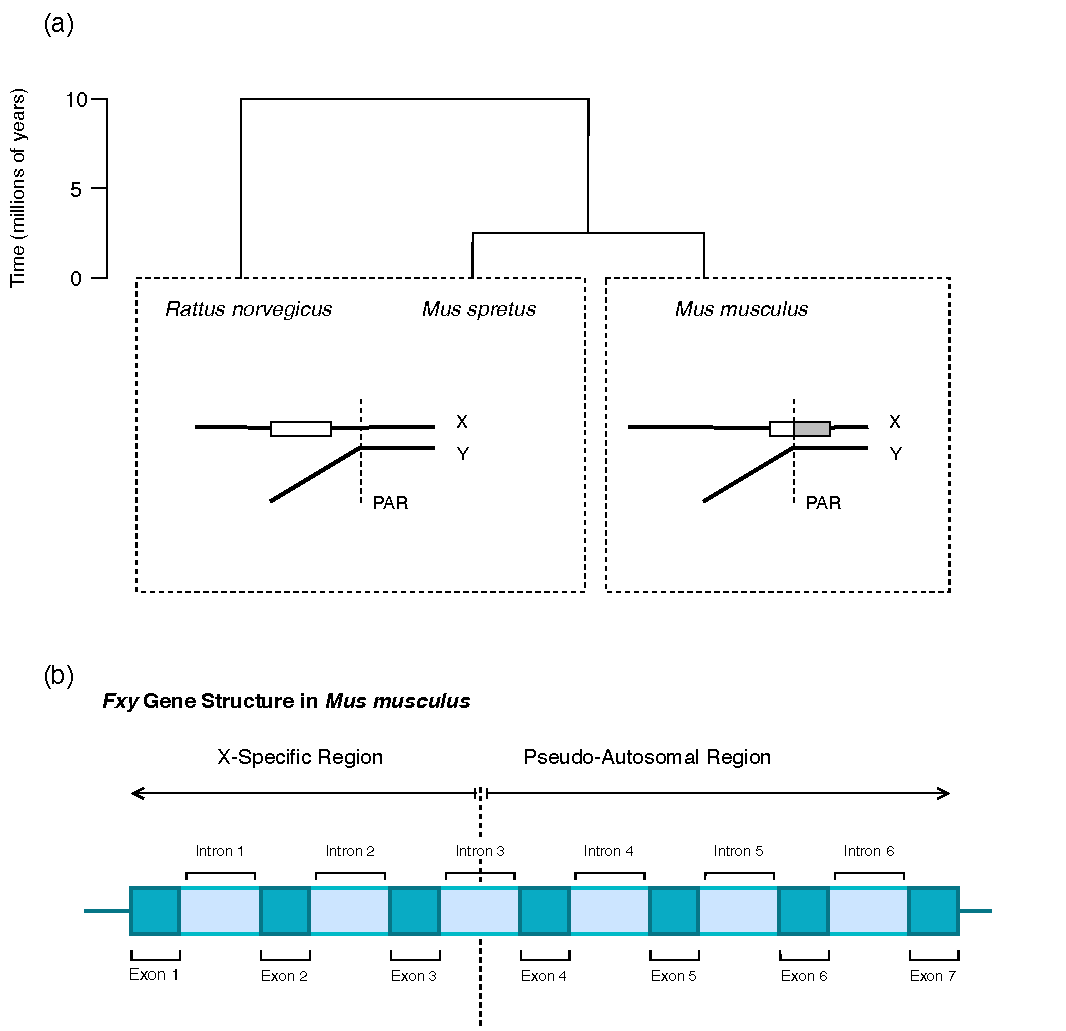
\includegraphics[width=\textwidth]{figures/diagrams/Fxy.pdf}
\caption[Evolutionary History of \textit{Fxy} in Rodents]{\textbf{Evolutionary History of \textit{Fxy} in Rodents}. \textbf{(a)} The \textit{Fxy} gene in \textit{M. musculus} was translocated from a X-specific position to a new position in which it overlaps with the PAR. The overlap in \textit{M. musculus} is shown as the shaded region of the gene, shown as a box. The divergence timescale is indicated in millions of years. In rodents and other mammals \textit{Fxy} is X-specific, suggesting translocation to the PAR in \textit{M. musculus} after divergence with \textit{M. spretus}, between 2-3 million years ago \citep[adapted from Figure 1][]{Galtier2007AdaptationEvolution}. \textbf{(b)} The structure of the \textit{Fxy} gene in \textit{M. musculus}. The $5'$ end of the gene, exons 1-3, are X-specific. The $3'$ end of the gene, exons 4-10, are positioned in the PAR. Note that for simplicity, exons beyond exon 7 are not shown in the structure. The boundary to the PAR falls in intron 3 of \textit{Fxy} \citep{Palmer1997AMice}. }
\label{fig:Fxy}
\end{figure}

The relative levels of purifying natural selection operating on a genomic segment allow for predictions of the magnitude of mutation disequilibrium. The abundance of functional elements in the genome outside of protein coding sequence (CDS) is very low \citep{Graur2013OnENCODE}. Accordingly, changes in intronic sequences are unlikely to be detrimental, making introns a useful neutral benchmark, or at least likely to be subject to a higher rate of mutation \citep{Graur2013OnENCODE}. Consequently, I expect CDS to exhibit a higher magnitude of mutation disequilibrium than intronic sequences that it flanks. For hetero-gametic sexes, you expect the chromosome that is hemizygous to be subjected to more stringent natural selection, because recessive deleterious alleles are exposed in the hemi-zygous sex \citep{Charlesworth1987TheAutosomes}. Given existing mutation disequilibrium, it is probable that an increased magnitude of purifying selection should slow the rate of convergence to equilibrium, and thus lead to a higher magnitude of disequilibrium. Accordingly, X-chromosome sequences should exhibit a higher magnitude of disequilibrium relative to autosomal sequences. 

Testing for mutation disequilibrium requires appropriate \gls{models} of sequence divergence. \Gls{Substitution models} impose varying assumptions on the divergence process, including, but not limited to: reversibility, that the process is identical to how it would appear if run in reverse; and \gls{stationarity}, the process is in \gls{equilibrium}. The evidence indicates the occurrence of, at the very least, historical changes in mutagenesis, in turn implying periods of mutation disequilibrium have existed in the past. However, this observation does not guarantee that disequilibrium persists. In order to interrogate this, I need models which are appropriate and fit for purpose. This is a non-reversible and non-stationary model for the alternate hypotheses (the existence of mutation disequilibrium), and a non-reversible but stationary model for the null (no mutation disequilibrium). 

\section{Previous work in detecting mutation disequilibrium}

Methods that are intended to tackle the statistical problem of testing for mutation disequilibrium have been proposed before, but not without limitations. \cite{Ababneh2006Matched-pairsSequences} introduced matched-pairs tests of homogeneity, looking at the internal and marginal symmetry of the nucleotide composition. These methods, however, are limited in power because they operate on pairs of sequences. To test for the existence of disequilibrium \cite{Squartini2008QuantifyingProcess} use a $\chi^2$-test comparing the current and equilibrium nucleotide distributions. The test proposed by \cite{Squartini2008QuantifyingProcess} appears to have a good theoretical basis, however, they do not evaluate whether the test statistic is consistent with the asymptotic approximations, or demonstrate that it behaves in a reliable manner. It remains unclear as to whether the methods are, in fact, reasonable. 

Methods of quantifying mutation disequilibrium have been developed, but do not measure all possible changes. \cite{Singh2009StrongDrosophila} introduced a time to equilibrium calculation of the GC content of a single \gls{edge} using a non-stationary but strand-symmetric process. \cite{Squartini2008QuantifyingProcess} introduced a method of quantifying disequilibrium using three indices, calculated from differences in the current and equilibrium nucleotide composition. Although defined for a general process, their work is demonstrated solely with a strand-symmetric model. Thus, both methods only consider changes in terms of GC content and consequently do not capture the complete scope of possible changes.

The detailed metadata now associated with genomes creates a wealth of new opportunities for methods development, enabling the inclusion of data of natural origins in experimental design. Traditional approaches to methods development relied near entirely on simulation studies for establishing the properties of a new method, and that is no longer adequate. The comprehensive understanding of the genetic underpinnings of methylation is what has provided the confidence of declaring that \textit{D. melanogaster} has recently lost this major mutagenic component in its genome. Therefore, it is a lineage that constitutes a positive control for the methods I seek to develop, and its sister taxa constitutes a relative negative control. The characterisation of the PAR in \textit{M. musculus} has allowed for the conjectured impact of translocation of the \textit{Fxy} gene. \textit{Fxy} provides another empirical control, the PAR located half is a positive control and the strictly X-linked half is the relative negative control. In addition to demonstrating consistency with asymptotic approximations and capturing the full scope of changes, these empirical controls are an essential extension of my methods relative to work previously done in the field. 

\section{Aims and scope}

In this work, I tackle the statistical problem of identifying the existence of mutation disequilibrium, its magnitude and whether it is equivalent between samples. Employing a complementary experimental design to interrogate natural occurrences of mutation disequilibrium on proposed positive controls, I address the following questions. Firstly, is there more mutation disequilibrium and does it have a greater magnitude in \textit{D. melanogaster} than in \textit{D. simulans}? Similarly, is this true for the PAR located component of \textit{Fxy} compared to the X-specific component in \textit{M. musculus}? Finally, I evaluate whether our own genome is in equilibrium. 

The results from the positive controls were striking in their consistency with the predictions. Consistent with the expectations of the neutral theory, genomic regions subjected to purifying natural selection are associated with higher incidence and magnitude of mutation disequilibrium. Results from the analysis of our genome indicate that the majority of our genome is not at equilibrium. I then discuss the implication of these results on our understanding of mutagenesis and future methods development in molecular biology. 
\newpage

\chapter{Methods}

\section{Data Sets}

\subsubsection{Microbial}

To establish the properties of my methods on alignments of taxa that range in their evolutionary divergence, I chose a widely used molecular marker of genetic diversity. Herein the Microbial data, this is a subset of GreneGenes, a database of consistent alignments of the 16S rRNA gene in microbes \citep{McDonald2012AnArchaeab}. The sequences are aligned using a customised alignment algorithm for ribosomal RNA that uses knowledge of secondary structure and conserved residues \citep{McDonald2012AnArchaea}. The Microbial data consists of 9702 alignments of species triples that were sampled from GreneGenes to get uniform representation of maximum Jensen-Shannon Divergence (JSD), details of the sampling process are described in \citep{Kaehler2015}. An important side effect of the sampling process is that a species can appear in more than one triple, so not each alignment is independent. The Microbial data was downloaded from Dryad data (\href{https://doi.org/10.5061/dryad.g7g0n}{https://doi.org/10.5061/dryad.g7g0n}).  

\subsubsection{Drosophila}

In order to test for elevated mutation disequilibrium in \textit{D. melanogaster}, I sampled alignments of \textit{D. melanogaster} genes with orthologs from closely related taxa: \textit{D. simulans} and \textit{D. yakubra}. Herein the Drosophila data, this contains 9237 alignments of one-to-one orthologs of protein coding sequence (CDS) obtained from \textit{flyDIVaS}, a database of curated \textit{D. melanogaster}-centric orthologous gene sets \citep{Stanley2016FlyDIVaS:Selection, Clark2007EvolutionPhylogeny}. The \textit{flyDIVaS} pipeline extracts protein-coding genes from the latest FlyBase release, identifying one-to-one orthologs using OrthoDB \citep{Zdobnov2021OrthoDBOrthologs}. Alignments of proteins are then performed using MUSCLE \citep{Edgar2004MUSCLE:Complexity}, which are backtranslated to CDS, filtered and masked. Further details of the sampling process are described in \citep{Stanley2016FlyDIVaS:Selection}. 

\subsubsection{Rodent}

To establish the impact of translocation to the PAR on the \textit{Fxy} gene in \textit{M. musculus}, I sampled one-to-one orthologs of \textit{Fxy} from \textit{M. spretus} and \textit{Rattus norvegicus}, in which \textit{Fxy} is X-linked. Intronic \textit{Fxy} sequence for all species was sampled using EnsemblDb3, an open-source python tool for querying Ensembl for related sequences \citep{HuttleyEnsembldb3}. The first eight introns of \textit{Fxy} were  aligned using the Cogent3 progressive nucleotide aligner with default settings \citep{Knight2007PyCogent:Sequence}. All alignments parameters were saved in a log file for which the indel length=0.1, indel rate=1e-10. 

\subsubsection{Great Apes}

Sampling CDS and introns from the same gene is an important part of experimental design. The human genome, as well as many of the great apes are extremely well curated genomic resource. Ensembl Compara \cite{Herrero2016EnsemblResources} contains annotated genome-wide species comparison data where annotation of orthology is quality controlled using synteny. Data for the Great Apes data set was sampled from Ensembl release 104 \citep{Howe2021Ensembl2021} using EnsemblDb3 \citep{HuttleyEnsembldb3} and homologsampler \citep{HuttleyHomologsampler}, open-source python tools for querying Ensembl for related sequences. I identified one-to-one orthologs of protein coding genes in chromosome 1 of \textit{Homo sapiens} (human), \textit{Pan troglodytes} (chimpanzee) and \textit{Gorilla gorilla} (gorilla) using homologsampler. From this gene list I sampled unaligned one-to-one orthologs of exons, which corresponds to the coding sequence from the canonical transcript. To sample the introns I sampled the genes with all exons masked, masked sequence is later filtered out giving an alignment of concatenated introns. The introns are aligned by Ensembl. I aligned CDS using the Cogent3 progressive codon aligner with default settings \citep{Knight2007PyCogent:Sequence}. The CDS alignment parameters were saved into a log file for which the indel length=0.1, indel rate=1e-10. 

\subsection{Data Filtering}

Substitution models are explicitly restricted to interchanges between nucleotide states, so annotated positions linked to other mutation types will be removed. This includes annotated gap characters, representing an insertion-deletion event, and simple tandem repeats, likely to evolve through strand slippage \citep{Levinson1987Slipped-strandEvolution}. For all CDS, I filtered to include sites corresponding to the third codon position only. Alignments that contained less than $300$ position after filtering were not included in the analyses. The number and summary stats of alignments pre and post filtering is included in Table (\ref{tab:seq_summary}). 

\begin{table}[ht]
\centering
\small
\setstretch{1.4}
\begin{tabularx}{\textwidth}{ 
  | >{\centering\arraybackslash}c
  | >{\arraybackslash}X 
  | >{\centering\arraybackslash}X 
  | >{\centering\arraybackslash}X 
  | >{\centering\arraybackslash}X 
  | >{\centering\arraybackslash}X | }
\hline
&  & \multicolumn{2}{c |}{\textbf{Raw}} & \multicolumn{2}{c |}{\textbf{Filtered}} \\ 
\hline
\textbf{Data Set} & Taxa & Number of Alignments & Min, Median, and Max Sequence Length (bp) & Number of Alignments & Min, Median, and Max Sequence Length (bp) \\

\hline

Microbial & * & - & - & 9,854 & 924, 1,138, 1,276  \\

\hline

Drosophila  & \hbox{\textbf{\textit{D. melanogaster},}} \hbox{\textbf{\textit{D. simulans},}} \textit{D. yakubra} & 9,237 & 120, 1,287, 26,952 & 5,944 & 300, 1,230, 26,676  \\

\hline

Rodent & \hbox{\textbf{\textit{M. musculus}},} \hbox{\textbf{\textit{M. spretus},}} \hbox{\textit{R. norvegicus}} & 8 & 4,948, 26,680.5, 57,007 & 8 & 834, 7,062, 42,742 \\ 

\hline

\shortstack{ \\ Great Ape \\ Introns} & \textbf{Human}, \textbf{Chimp}, Gorilla & 1,481 & 103, 9,679, 298,974 & 1,406 & 302, 7,723.5, $274,635$ \\

\hline

\shortstack{ \\ Great Ape \\ CDS} & \textbf{Human}, \textbf{Chimp}, Gorilla & 1,683 & 165, 1,365, 26,775 & 1,182 & 300, 545.5, 8,601 \\

\hline

\end{tabularx}
\caption{\textbf{Summary of Data Sets.} The ingroup edges for each set of taxa are bolded. \\ \textbf{*} The Microbial data set is comprised of alignments of the same sequence, but for different triads of taxa. }
\label{tab:seq_summary}
\end{table}


I can exemplify the filtering process using dotplots. A dotplot is a way of visualising the relatedness between biological sequences \citep{Gibbs1970TheSequences}. In this case, the X and Y axes correspond to a nucleotide sequence, each dot on the plot indicated where the  nucleotide is identical between the two. Long stretches of identity between the two sequences form a diagonal. Using a psuedorandom algorithm I selected an alignment from both the Great Ape CDS and Intronic data sets to exemplify this filtering process, shown in Figure (ref). 



\section{Models}

In this work I will use two continuous-time models, General Nucleotide (GN), and General Stationary (GS), and one discrete-time model, the Barry and Hartigan (BH) model. 

\subsubsection{GS}

\subsubsection{GNS}


\subsubsection{GTR}


\subsubsection{BH}
GN is a non-stationary nucleotide model for which time-homogeneity between nodes in the tree is the only required constraint \citep{Kaehler2015}. GNS is a stationary nucleotide model, formulated by Von Bing Yap and Gavin Huttley (Personal Communication). The BH model is a general discrete-time Markov process for nucleotides \citep{Barry1987StatisticalEvolution}. The assumptions for each can be found in table \ref{model_assumptions}.
\begin{table}[htbp]
\centering
\begin{tabularx}{0.7\textwidth}{ 
  | >{\centering\arraybackslash}c 
  | >{\centering\arraybackslash}X 
  | >{\centering\arraybackslash}X  
  | >{\centering\arraybackslash}X | }
\hline  
\textbf{Assumption} & \textbf{BH} & \textbf{GN} & \textbf{GS}  \\
\hline 
    Reversibility & - & - & -  \\
    Stationarity & - & - & \checkmark  \\
    Time-Homogeneity  & - & \checkmark & \checkmark \\
    Independent sites & \checkmark & \checkmark & \checkmark\\ 
\hline 
\end{tabularx}
\caption{Markov process assumptions}
\label{model_assumptions}

\end{table}




\subsection{General Nucleotide Markov}

\section{Defining Novel Statistical Measures}

\section{Maximum Likelihood}

For some data, the likelihood of a hypothesis is the probability of the data given that hypothesis. For likelihoods involving substitution models, the tree topology and the values of free parameters are these hypotheses \cite{Lio1998ModelsPhylogeny}. ML methods `fit' a model by returning the model parameters that produce the highest probability of generating the observed sequence data \citep{Edwards1972Likelihood, Felsenstein1981EvolutionaryApproach}. ML is a powerful framework for determining whether there is significant improvement between nested models \cite{Goldman1993StatisticalSubstitution}. One `null' model is considered nested in another if it can be specified simply by imposing restrictions on the parameters of the `alternate' model. For the models of interest, GNS is nested within GN.

A likelihood ratio test (LRT) is a method of comparing nested models \citep{Goldman1993StatisticalSubstitution}. It is a test of whether additional components unique to the alternate model cause a significant improvement in the description of the data \cite{Goldman1993StatisticalSubstitution}. Practically, this involves comparing likelihoods between models, giving a LRT statistic. Suppose the null model is appropriate and the length of the alignment is adequate. In that case, the LRT statistic will be $\chi^2_{df}$ distributed with degrees freedom (df) equal to the difference in the number of free parameter between the models \citep{Lindgren1993StatisticalTheory, Silvey1975StatisticalInference, Kendall1979The2}.

\subsection{Test of Existence}

To achieve this aim I have designed a Likelihood Ratio Test (LRT). The predominant method for examining aspects of sequences' evolution is through the use of \glspl{Substitution model}. \Gls{Maximum Likelihood} methods allow for measuring the support for a hypothesis, (in this case, a \gls{model}), given some data. Whether one hypothesis is better supported than another can be evaluated by using an LRT. Two models fundamental for my LRT are General Nucleotide (GN) and General Nucleotide Stationary (GNS). Their point of difference is that the parameters of a GNS rate matrix must satisfy $\pi\mathbf{Q}=0$, i.e., the process is constrained to be stationary (and thus in equilibrium). Consider an LRT in which GNS is the null and GN is the alternate. If we reject the null, we may conclude that the sequences are more likely to have been generated by a process which is not yet stationary, as this is the only component unique to the alternate.

An LRT as described above is too naive for my objective to test for equilibrium in a single lineage. For a model to be \gls{identifiable} requires an alignment of at least three sequences \cite{Chang1996FullConsistency}. Consequently, a significant result for such an LRT will not reveal which of the taxa is causing the rejection of the null. To test for disequilibrium in a single \gls{edge} requires  modelling a continuous-time process on the edge of interest (herein the foreground edge) and assuming discrete-time processes for the other edges (herein the background edges) \cite{Verbyla2013TheSubstitution}. A discrete-time process is more general (fewer assumptions) than even the GN, making it the ideal background. 

Using mixed discrete- and continuous-time Markov processes, I can test for disequilibrium on a single edge. For such an LRT, the foreground edge assumes GNS for the null, and GN for the alternate. Both hypotheses assume a Barry and Hartigan (BH) model, the most commonly implemented discrete-time process, for the background edges. The modelling of the foreground edge, set apart by the assumption of stationarity, is the only point of difference between hypotheses. For this LRT, a rejection of the null means that the foreground edge was described significantly better with a non-stationary process. Such a result suggests disequilibrium precisely in the foreground edge. Put explicitly, the test will be between the following hypotheses:\\ $\mathbf{H_0}$: the foreground evolved according to the \textbf{GNS}, the background according to BH. \\ $\mathbf{H_1}$: the foreground evolved according to the \textbf{GN}, the background according to BH.\\
\noindent Herein all model fits assume mixed discrete- and continuous-time Markov processes, and a BH process is always assumed for the background edges. For brevity, I will refer to a model by the process assumed on the foreground edge.

\begin{figure}[htbp]
\centering
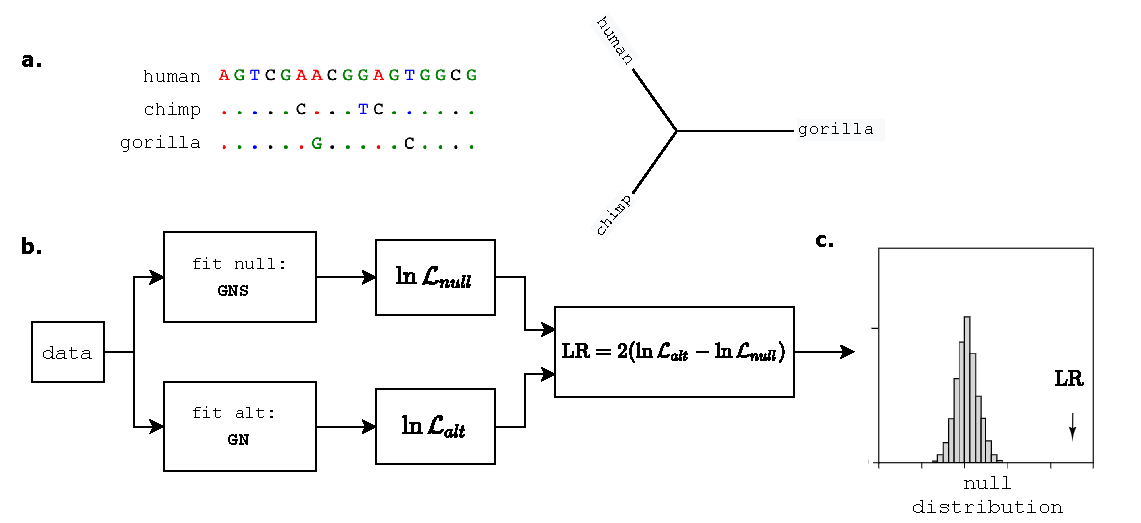
\includegraphics[width=\textwidth]{figures/diagrams/LRT.pdf}
\caption{\textbf{Likelihood Ratio Test.} \textbf{a}, The data: an alignment of orthologous sequences for human, chimp and gorilla, and a phylogenetic tree indicating the relationship between taxa. \textbf{b}, A LRT comparing substitution models, GNS is the null and GN is the alternate. The log-likelihood ($\ln\mathcal{L}$) for each model is obtained via fitting. The likelihood ratio (LR), is the ratio of the $\ln\mathcal{L}$ of the two models. \textbf{c}, the LR statistic is compared to the null distribution. In this case the statistic exceeds the distribution of values we would expect if the null was true, we would thus conclude that process is described significantly better with the alternate (GN) process.}
\label{fig:lrt}
\end{figure}

\subsection{Tests of Equivalence of Process}

For a single alignment of three taxa, a split continuous- and discrete-time model can be specified by the following set of parameters: $( \bm{Q}_{fg}, \bm{P}_{bg1}, \bm{P}_{bg2}, \pi_{0}, b ) $ where $\bm{Q}_{fg}$ is a continuous-time rate matrix describing the foreground edge,  $\bm{P}_{bg1}$ and $\bm{P}_{bg2}$ are discrete-time probability substitution matrices each describing one of the background edges, $\pi_{0}$ is the motif probabilities in the most recent common ancestor, and $b$ is the branch length corresponding to the foreground edge. 

For the adjacent Equivalence of Process test (aEOP) between two alignment $\alpha$ and $\beta$, the null hypothesis constrains both alignments to have the same root motif probabilities and the same rate matrix on the foreground edge, i.e.,  \\
$H_0:$ $\bm{Q}_{fg}(\alpha) = \bm{Q}_{fg}(\beta)$ and $\pi_0(\beta) = \pi_0(\alpha)$. \\
\noindent
The alternate hypothesis allows all parameters to be independent between alignments. 

The temporal Equivalence of Process test (tEOP) is between two edges of the same aligned sequence. In this case, there are two edges of interest, so the process is modelled with all edges as continuous time process. Such a model is specified by the following set of parameters: $( \bm{Q}_{fg1}, \bm{Q}_{fg2}, \bm{Q}_{bg}, \pi_{0}, b_{fg1}, b_{fg2}, b_{bg1}) $, where $\bm{Q}_{fg1}$ and $\bm{Q}_{fg2}$ are continuous-time rate matrices each describing on of the foreground edges,  $\bm{Q}_{bg}$ is a continuous-time rate matrix describing the background edge, $\pi_{0}$ is the motif probabilities in the most recent common ancestor, and $ b_{fg1}, b_{fg2}, b_{fg1}$ is the branch length corresponding to the foreground edge. The null hypothesis constrains both foreground edges to have the same rate matrix, i.e., \\
$H_0:$ $\bm{Q}_{fg1} = \bm{Q}_{fg2}$  \\ 
The alternate hypothesis allows all parameters to be independent. 

\subsection{Bootstrapping Procedure}

\section{Experimental Design}

\subsection{Choosing Seed Alignments}
I require alignments simulated in accordance with a GNS process. One way to obtain data evolving under a GNS process is to exploit the fact that even a non-stationary process will converge to its stationary nucleotide distribution (herein $\pi_{\infty}$) as time goes to infinity. Essentially, I can obtain a GN model from real data, derive its corresponding $\pi_{\infty}$ and use those two things to define a stationary process. The process can be modified to model the background edges as discrete, and I can simulate alignments according to such a specification. This is my chosen simulation method as the resulting alignments are generated from parameters of real data. 

I must consider how the properties of the alignment used for simulation may affect the application of my methods. To address this requires deciding the features of an alignment that may be significant and finding measures that characterise them. I can then choose a selection of alignments that vary systematically by these measures. From each alignment, I can create a data set, resulting in a collection of data sets that differ in a way that reflects the natural variation of real sequence data. Using carefully diversified data allows for a thorough interrogation of my methods and determines how their properties may change when applied to different types of data.

An important measure I require is that of non-stationarity. A direct consequence of a non-stationary process is a change in base composition over time. As follows, an indication of the degree of historical non-stationarity can be obtained from the difference in compositions between sequences in the same alignment. It is worth noting that studies of compositional data often require representation using Aitchison geometry. This representation allows for a consideration of the vulnerability of a composition to the sample it comes from. However, the composition of bases can also be considered as a probability distribution (i.e., $\pi = [\pi_T,\, \pi_G, \, \pi_C, \, \pi_A]$, such that $\pi_i$ where $i= \mathrm{T}, \mathrm{G}, \mathrm{C}, \mathrm{A}$ is the probability of observing the state $i$). In the case of comparing probability distributions, several measures can be used. My selected measure is an information theoretic measure known as Jensen-Shannon Divergence (JSD). JSD measures the similarity between probability distributions. JSD was chosen as it can accommodate multiple distributions, allowing us to apply it to more than two sequences if needed. Additionally, it has an associated true metric, satisfying important mathematical properties (e.g., the triangle inequality). 

A probability distribution also has an associated information content, measured using entropy. Entropy is a fundamental quantity that indicates, in our case, the evenness of base composition. For example, $\pi =[1,\, 0,\, 0,\, 0]$  (a single nucleotide) has zero entropy whilst  $\pi =[0.25,\, 0.25,\, 0.25,\, 0.25]$ (equifrequent nucleotides) has the maximum possible entropy for 4 states. As a measure of compositional diversity, it captures an essential feature of the mode of evolution. For example, an edge that is highly \gls{strand-asymmetric} would have lower entropy than a \gls{strand-symmetric} edge. The base composition may affect the properties of my developed methods. One example being $T_{50}$ for which base composition is used in its computation. Accordingly, the impact of compositions with different entropy is an important feature to consider in the process of method development.

I will approximate the stability of the process using the condition number of the foreground rate matrix. It is important to derive data from numerically stable processes. If a process falls within the scope of being numerically unstable, (meaning computers are poorly equipped to evaluate it using standard settings), I need to be aware of this so I can select a more numerically stable method. An indication of numerical stability is the eigenvector matrix condition number. A matrix condition number is an approximation of the worst case relative change in derivations, for a relative change in the input. For a continuous-time process, the transition rate matrix $\mathrm{Q}$, specifies the instantaneous rates of exchanges between states. $\mathrm{Q}$ is foundational to a given substitution model. The eigendecomposition of $\mathrm{Q}$ is a representation of $\mathrm{Q}$ in terms of its eigenvalues and eigenvectors. Eigendecomposition is fundamental to many methods that I am using and developing (e.g., deriving $\pi_{\infty}$). As an indication of the suitability of a matrix to decomposition, I will use the eigenvector matrix condition number to approximate the numerical stability of a process.

I chose four microbial alignments to generate synthetic data sets and refer to these as seed alignments. As previously stated, I expect that JSD, entropy, and condition number may affect the numerical and or statistical properties of the developed methods. To derive data from numerically stable processes, the seed alignments are chosen from a subset of alignments where the eigenvector condition number is low ($<1.5$). To capture the extent of naturally occurring diversity (measured by JSD) and compositional diversity (measured by entropy), the seed alignments chosen represent the permutations of those extremes. These are: high JSD, low entropy; high JSD, high entropy; low JSD, low entropy; low JSD, high entropy. 

\subsection{Generating Synthetic Alignments that are Stationary, but not Reversible}
I expect the properties of my test to be affected by the number of substitution events that distinguish the sequences in an alignment. The mathematical proof that LRT statistics are $\chi^{2}$ distributed assumes infinite data, that is the alignment is infinitely long. Although it has been shown that a few hundred base pairs can be sufficient for the $\chi^{2}$ to be accurate, this length is ultimately dependent on the number of substitution events \cite{Ota2000AppropriateParameters}. I can increase the number of events in a simulated alignment in two ways, (1) increase the length of the alignment, (2) increase the \gls{branch length} of the tree (increased divergence time). 

It is necessary to determine how my methods are affected by the length of the alignment. I have done this by simulating multiple data sets differing in alignment length for all four seeds. The lengths were chosen to be representative of alignment lengths of my biological application. The shortest sequences I will be using are protein coding genes, for which the average length (using just the 3rd codon position) is about 300bp. For each of the four seeds, I generated data sets of alignment length 300, 3,000, and 30,000.   

It is also necessary to determine the influence of increased branch length. When simulating alignments, I can alter the branch lengths of the generating function. This is a capability that allows me to create synthetic alignments specified by the same process (same $\mathrm{Q}$), but with an increased term of divergence. To address how branch length affects the test, I simulated data sets with an increased branch length for all four seeds. The genetic distance ($d$) (or branch length) is a measure of the expected number of nucleotide substitutions per site. The maximum branch length in my application data sets will be about $d=0.6$. For the long branch simulations, I scaled the tree by a factor of 3. However, branch lengths were capped at $d=0.6$ and the remaining branch lengths were reduced proportionally. 

Each simulation set consisted of 1,000 synthetic alignments. The synthetic alignments are generated from the same function, derived from the parameter estimates from one seed alignment. The simulation process that was performed is described in Figure \ref{fig:simulating_alns}.

\begin{figure}[!ht]
\centering
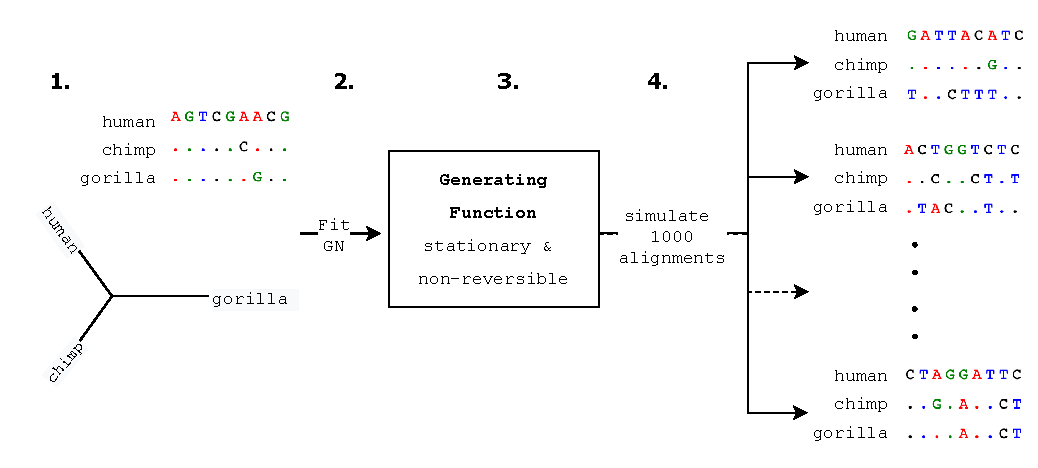
\includegraphics[width=\textwidth]{figures/diagrams/simulating_alns.pdf}
\caption{Creating synthetic data sets whose evolution was stationary but not reversible. \textbf{1,} select seed alignment, \textbf{2}, fit GN mixed model and extract model parameter estimates, \textbf{3}, define generating function using parameter estimates altered to be stationary, \textbf{4}, generate 1000 alignments of length $n$ and branch length scaled by $b$. For all 4 seeds this was performed for n = 300, 3000, 30000, and for each n, b = 1 and 3.}
\label{fig:simulating_alns}
\end{figure}

\section{Algorithmic Implementation}


\newpage

\chapter{Results}

% PAST TENSE when describing work that I have done and each result section should refer to the aim that it is tackling

The aim of the methods described in this thesis is to provide tools to query the disequilibrium of sequence evolution. Described in this chapter is the characterisation of the developed methods. I present the application of the test of existence and test of consistency to simulated data. Additionally, I present two new statistics for measuring the magnitude of disequilibrium. I evaluated these statistics on simulated data. Having selected statistical measures based of validation with data consistent with the null hypothesis, I applied my methods to naturally occurring cases of the alternate hypothesis aiming to validate whether they do, in fact, reflect an elevated level of disequilibrium. I report the application of my methods to two biological cases with striking prior evidence for recent perturbations affecting: an entire genome (loss of DNA methylation in \textit{D. melanogaster}); or, a small genomic segment (\textit{Fxy} in \textit{M. musculus}). I find that the methods are consistent with prior predictions made with knowledge of mechanism alone.  

\section{Developing and validating the methods}


A process of validation was applied to each method. A simple specification of methods is not enough, it is necessary to determine how it behaves and that it behaves in a way that matches up with the expectation when how the data is generated is known. There is an infinite number of ways in which things can be out of equilibrium, but the number of ways in which they can be in equilibrium is a lot more restrictive. Since I am interested in departures from being in equilibrium, that’s the condition set that I have imposed in developing the methods. Below I describe the intent of a particular statistic, then describe how it was developed.

\subsubsection*{The best method of model fitting is without initialisation}

It is important that the best possible methods of model fitting are chosen. The test of existence seeks to determine whether the process is described significantly better by a non-stationary process. Formally, the test of existence is an LRT between the following hypotheses:\\ $\mathbf{H_0}$: the foreground evolved according to the \textbf{GNS}, the background according to BH. \\ $\mathbf{H_1}$: the foreground evolved according to the \textbf{GN}, the background according to BH.\\
A necessary precursor to any application of the test is to establish maximal fits of the models. Additionally, the process of fitting a model to an alignment is the most time-consuming method routinely used in my project. I have sought to identify the quickest possible method that yields a maximised likelihood. 

For this, I conducted an initialisation experiment that makes use of a property of nested models. For nested models, it is guaranteed that the likelihood for the alternate will be greater or equal to that for the null. General Time-Reversible (GTR) is the most general time-reversible process and is required for my initialisation experiment. GTR is nested in GNS, which in turn is nested in GN. When a model is not maximally fit, the optimisation methods have failed to find the global maximum. Such is referred to as a local maximum, where they are higher points elsewhere but not nearby. In such cases, getting parameter estimates from a nested model fit to use as initial estimates may aid the optimisation in escaping a local maximum. I also wish to establish whether there is a speed gain in initialised model fits compared to uninitialised fits. Theoretically, if given starting values close to the optimal, this may reduce the time it takes to get there. 

For all synthetic data sets, I tested whether initialisation improved the model fitting process. The initialised method fit models in order of increasing generality (GTR, GNS, GN). Importantly, parameter estimates for each model were obtained from the previous model. The uninitialised method fit GNS and GN separately. The maximum likelihood estimates between uninitialised and initialised fits were compared for the models (e.g., uninitialised GN vs initialised GN). The time taken for each fitting process was recorded.  

The initialisation experiment revealed that there are no intrinsic problems with the fitting process for GN or GNS. A fit was considered non-maximal if the log-likelihood from the initialised method was higher than that of the uninitialised method. There were no occurrences of non-maximal fits for any of the synthetic alignments. Initialised fits which were faster than the corresponding uninitialised fits were rare, occurring at a rate of about ~1\%. These results suggest that the best method of fitting for both models is without initialisation.

\subsubsection*{The LRT for Existence with parametric bootstrapping provided a robust estimation of significance}

To determine whether a given LRT statistic is significant requires establishing the appropriate null distribution. Statistical theory states that under certain conditions, the LRT statistic will be $\chi^2_{df}$ distributed with degrees freedom (df) equal to the difference in the number of free parameters between the models. In which case, one can obtain the p-values for a given LRT statistic simply from the analytical distribution. However, the behaviour of my test with real finite data is unknown. When considering the use of mixed discrete- and continuous-time Markov process is a deviation from convention, it is especially important to establish whether the test statistic is consistent with theoretical expectations. 

The distribution is closer to theoretical expectations for longer sequences, depicted in Figure \ref{fig:synthetic/lrt/197113-long_seq}. The figure shows data generated from the same high JSD, high entropy seed process, however, the results for all seeds were very similar, see appendix Figure \ref{fig:synthetic/lrt/all-seeds}. For alignments of length 300bp, shown in Figure \ref{fig:synthetic/lrt/197113-long_seq}a, the distribution of LRT statistic yields an excess of small p-values. Consequently, the data points of the Quantile-Quantile plot fall well below the diagonal line. Owing to increasing the power of the test, the distribution of p-values for longer alignments, illustrated in Figure \ref{fig:synthetic/lrt/197113-long_seq}b, is less skewed. Overall, the data points fall much closer to the diagonal line. It is worth noting that consistency with the theoretical distribution is most important for the smaller p-values. In Figure \ref{fig:synthetic/lrt/197113-long_seq}b, for quantiles corresponding to a significant test statistic (i.e. the bottom left corner where $p<0.05$), the distribution is very close to the theoretical distribution. This means that the chance of a false-positive is more or less in line with statistical expectations (5\%). Now, consider the distribution of p-values for $p>0.05$. Even though the distribution is not uniform, using the $\chi^{2}$ distribution, a non-significant result would still yield a non-significant p-value (true-negative). Thus, for some longer alignments, it may be suitable to assume the LRT statistics are $\chi^{2}$ distributed and in turn, obtain the p-value simply from analytical distribution. 

\begin{figure}[htbp]
\centering
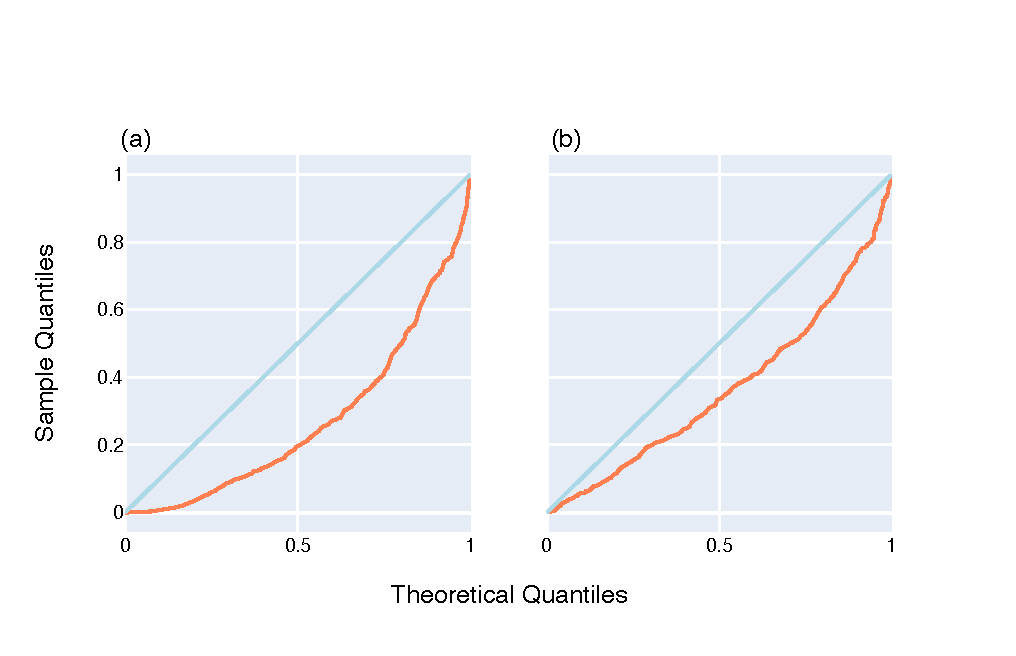
\includegraphics[width=\textwidth]{figures/plots/synthetic/lrt/197113_332182_17210-long_seq.pdf}
\caption[Increasing the length of the alignments gives a distribution of $\hat p-$ values closer, but not consistent with theoretical expectations]{\textbf{Increasing the length of the alignments gives a distribution of $\hat p-$ values closer, but not consistent with theoretical expectations.} The Quantile-Quantile (Q-Q) plots compare the $\hat p$-value distribution of the test for existence in stationary simulated data to the uniform distribution (pink line). Theoretical expectation is illustrated by the diagonal (blue line). Q-Q plot for \textbf{(a)} synthetic alignments of length $300$bp, \textbf{(b)}, synthetic alignments of length $30,000$bp. Each data set contains 1,000 synthetic stationary alignments. Both data sets shown are generated from the same high JSD, high entropy seed. The other seeds exhibited the same pattern, the result is shown in the appendix Figure \ref{fig:synthetic/lrt/all-seeds}.}
\label{fig:synthetic/lrt/197113-long_seq}
\end{figure}

The exploration with synthetic data clearly informs the application of my test. Firstly, the results of the initialisation experiment show there is no intrinsic fitting problems. As such, model fitting in all cases will be done without initialised parameter estimates. The results in Figure \ref{fig:synthetic/lrt/197113-long_seq} demonstrate that I cannot assume the LRT statistic to be $\chi^{2}$ distributed. As conventional asymptotic approximations to the LRT distribution are shown not to apply, significance levels will need to be assessed via a parametric bootstrap. 

\subsubsection*{A transformed $\nabla$ statistic exhibited robust behaviour under the null}

The statistic $\nabla$ is a measure of the speed of convergence of the actual process to equilibrium. Consider a process operating on a single edge of a phylogenetic tree for a time interval of length $t$, for which the frequencies of nucleotides at the root is $\pi_0$ and the rate matrix on the edge is $Q$. The nucleotide distribution at $t$ is $\pi(t) = \pi_{0} \cdot e^{Qt}$. For a stationary process, this simplifies to $\pi(t) = \pi_{0}$. Under weak assumptions, a non-stationary process will converge to a stationary process, for which $\pi$ remains unchanged over time. Thus, I can describe the speed of this convergence with the rate of change of $\pi(t)$. In other words, the derivative of $\pi$ with respect to $t$,
\begin{equation}
\label{eq:dpi/dt}
\frac{\partial \pi}{\partial t}(t) = \pi_{0} \cdot Q \cdot e^{Qt}.
\end{equation}

To describe the magnitude of a vector in a single value, it is natural to take its length. Accordingly, the $\nabla$ statistic is defined as follows,
\begin{equation}
\label{eq:len-dpi/dt}
\nabla = ||\frac{\partial \pi}{\partial t}(t)|| =|| \pi_{0} \cdot Q \cdot e^{Qt}||.
\end{equation}
$\nabla$ is the magnitude of the rate of change of $\pi(t)$. For a stationary process, for which by definition $\pi$ does not change over time, $\nabla = 0$. For a non-stationary process, as the process approaches equilibrium, $\nabla$ will asymptote to $0$. For a given non-stationary process that converges monotonically to equilibrium, $\nabla$ must increase the further one moves from equilibrium. The algorithm used to calculate $\nabla$ is presented in Algorithm \ref{alg:convergence}.

\begin{algorithm}[ht!]
\caption[Algorithm]{Calculating $\nabla$}
\label{alg:convergence}
\begin{minted}{python}
def convergence(pi_0, Q, t):

    pi_deriv = dot(pi_0, dot(Q, expm(Q * t)))
    conv = norm(pi_deriv)

    return conv
\end{minted}
\end{algorithm}


The $\nabla$ statistic required a transformation to address bias introduced in short sequences. Presented in Figure \ref{fig:synthetic/d-conv-vs-conv/HighJSDHighEntropy}a are the distributions of $\hat \nabla$ in simulated data sets generated by the same stationary seed, but for alignments of length 300, 3,000, and 30,000. Figure \ref{fig:synthetic/d-conv-vs-conv/HighJSDHighEntropy}a shows that not only was there more variation in $\hat \nabla$ for the shorter alignments, but the location of the mean differs between lengths. The High JSD, High Entropy seed is shown in Figure \ref{fig:synthetic/d-conv-vs-conv/HighJSDHighEntropy}a, however, this result was the same for all seeds, included in the appendix (see Figure \ref{fig:synthetic/conv/all_seeds}). Empirical applications must compare statistics between sequences of different lengths, for which the $\nabla$ statistic requires a transformation. 

\begin{figure}[htbp]
\centering
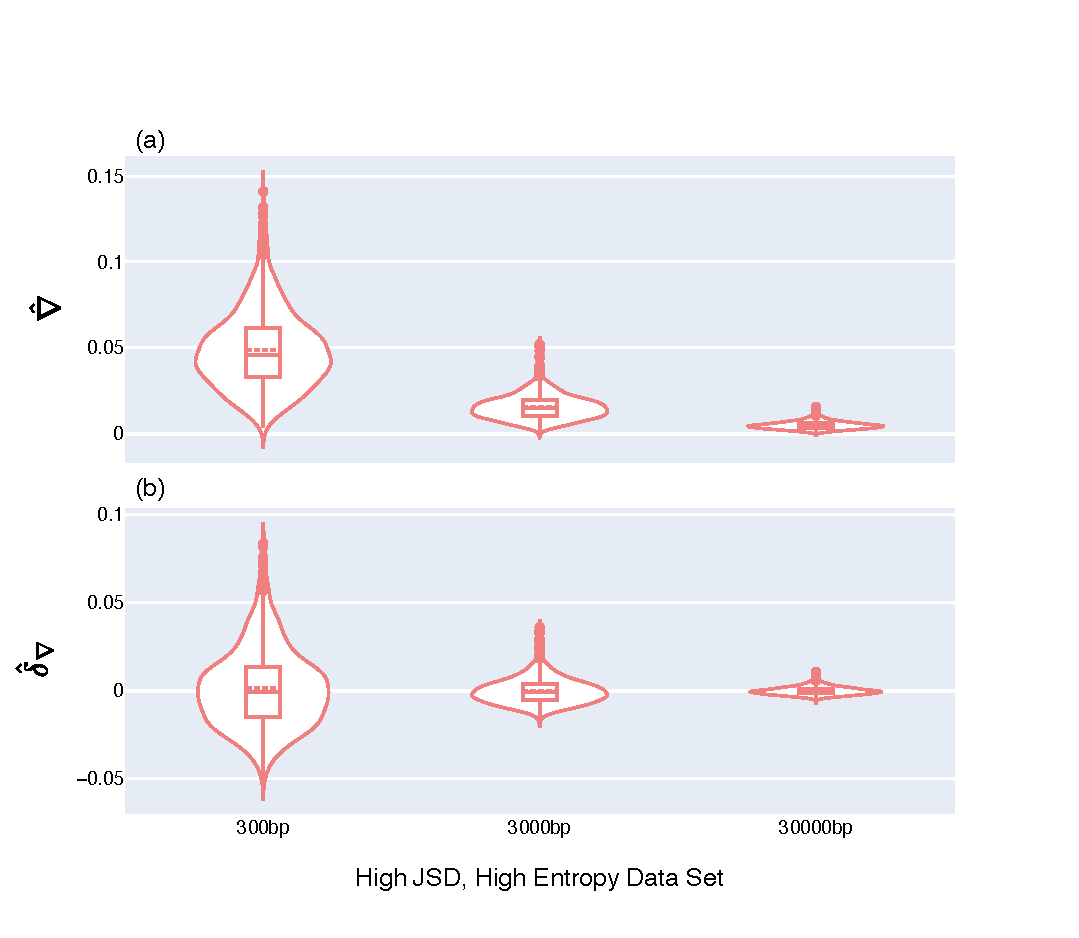
\includegraphics[width=\textwidth]{figures/plots/synthetic/d-conv-vs-conv/High JSD, High Entropy.pdf}
\caption{\textbf{The transformed statistic, $\delta_\nabla$, corrects for error introduced by the length of the alignment.} The violin plots show the distribution of $\hat \delta_\nabla$ for simulated data sets of alignment length 300, 3,000, and 30,000. \textbf{(a)} The original statistic, $\nabla$, had both a higher level of variation and a higher expected value in shorter sequences. \textbf{(b)} The transformed statistic $\delta_\nabla$ corrects for the location of the expected value only. The variation in shorter sequences remains, however, the mean for alignments of all lengths is centred on zero. Each data set contains 1,000 synthetic stationary alignments. The High JSD, High Entropy seed is shown, however, this result was the same for all seeds, included in the appendix (see Figure \ref{fig:synthetic/conv/all_seeds}). }
\label{fig:synthetic/d-conv-vs-conv/HighJSDHighEntropy}
\end{figure}

The selected transformation, denoted $\delta_\nabla$, adjusted for location only, ensuring the expected value was zero when the null was true. For a given alignment, $\hat \delta_\nabla$ is the difference between the observed $\hat \nabla$ and the mean of  $\hat \nabla$ of synthetic alignments generated under the null, put explicitly, $\delta_\nabla =  \nabla - \mu_{\nabla{null}}.$ Presented in Figure \ref{fig:synthetic/d-conv-vs-conv/HighJSDHighEntropy}b are the distributions of $\hat \delta_\nabla$ in simulated data sets again generated by the High JSD, High Entropy seed for alignments of length 300, 3,000, and 30,000. \ref{fig:synthetic/d-conv-vs-conv/HighJSDHighEntropy}b shows that the expected value of the transformed $\delta_\nabla$ statistic is close to zero when the null is true. Although there is more variation in the shorter sequences, this simple method of transformation was chosen because the statistic retains the same units as the untransformed statistic. Normality?

The $\delta_\nabla$ statistic increases with a known marker of historic disequilibrium. JSD is an information theoretic measure of the difference between probability distributions. Therefore, the JSD between two edges of a tree is an indication of the level of historic disequilibrium in one or more of the lineages. The $\delta_\nabla$ statistic has a strong positive relationship with the JSD between ingroup edges for taxa from the microbial data set, illustrated in Figure \ref{fig:microbial/d-conv/JSD}. This relationship is very encouraging as it supports that $\delta_\nabla$ is in fact measuring what it is intended to measure, mutation disequilibrium. 

\begin{figure}[htbp]
\centering
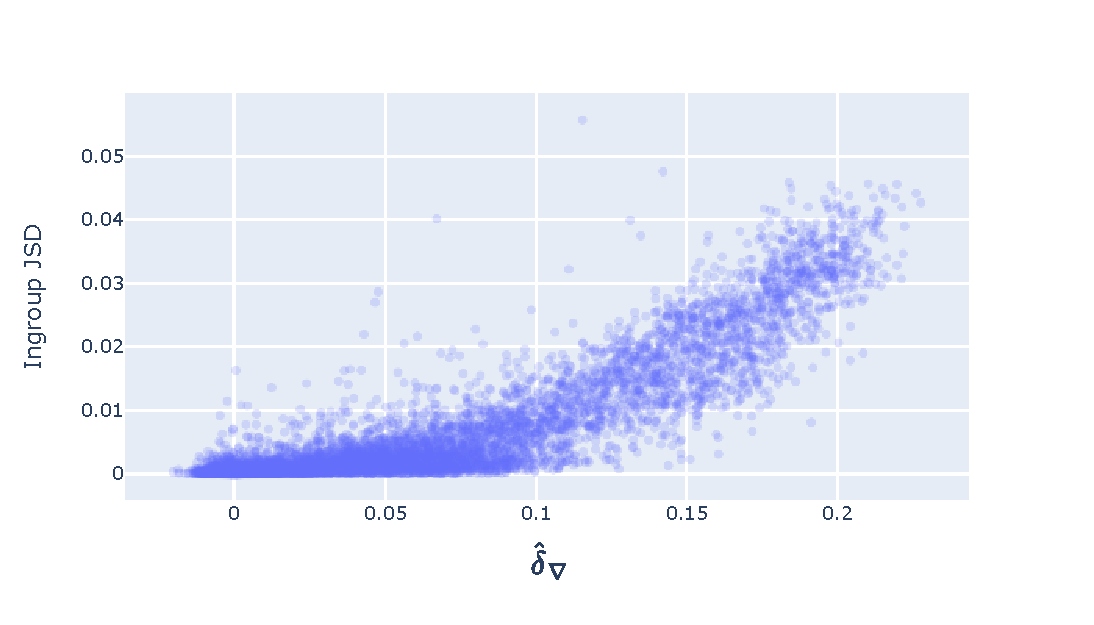
\includegraphics[width=\textwidth]{figures/plots/microbial/d-conv-JSD.pdf}
\caption{\textbf{The $\hat\delta_\nabla$ statistic increased with a marker of historic disequilibrium.} The scatter plots shows magnitude of disequilibrium measure by $\hat\delta_\nabla$ and the JSD between ingroup taxa for the observed Microbial data set. The Microbial data set comprises 9702 alignments where the level of disequilibrium is expected to vary.}
\label{fig:microbial/d-conv/JSD}
\end{figure}

\subsubsection*{The $T_{50}$ statistic exhibited paradoxical propertied that prevented interpretation}

A seemingly natural way to describe disequilibrium in a system is by its proximity to equilibrium. As previously stated, for a process in disequilibrium, as time goes to infinity, its nucleotide distribution will converge to $\pi_\infty$, its equilibrium distribution. This can be expressed mathematically as 
$$\pi_\infty = \lim_{t \to \infty}\pi \cdot e^{\mathbf{Q}t}.$$ 
This property manifests in other situations, for example, the decay of a radioactive element. In those fields the problem of quantification is solved by expressing in terms of an arbitrarily chosen metric, half-life, the time taken until half of the element's original mass is left. $T_{50}$ is defined equivalently. ${T_{50}}$ is a measure of the distance to halfway to $\pi_\infty$, measured in terms of the expected number of substitutions. The algorithm used to calculate $T_{50}$ is presented in Algorithm \ref{alg:t50}.

\begin{algorithm}[ht!]
\caption[Algorithm]{Calculating $T_{50}$}
\label{alg:t50}
\begin{minted}{python}
class T50:
    def __init__(self, Q, pi_0, func=jsm):
        """
        func
            a callback function that takes two probability vectors
            and returns a "distance". Defaults to Jensen-Shannon metric.
        """
        self.Q = Q
        self.pi_0 = pi_0
        self.pi_inf = self.get_stat_pi()
        self.dist_halfway = func(self.pi_0, self.pi_inf) / 2
        self.tau = 1
        self.dist_func = func

    def get_stat_pi(self):
        return get_stat_pi_via_brute(expm(self.Q), self.pi_0)

    def estimate_t50(self):
        ens_curr = expected_number_subs(self.pi_0, self.Q, 1)
        self.tau = minimise(
            self,
            xinit=self.tau,
            bounds=([1], [1e10]),
            local=True,
            show_progress=False,
            tolerance=1e-8,
        )
        ens_50 = expected_number_subs(self.pi_0, self.Q, self.tau)
        return ens_50 - ens_curr

    def distance_from_pi_zero(self, pi):
        return self.dist_func(self.pi_0, pi)

    def __call__(self, tau):
        pi_tau = dot(self.pi_0, expm(self.Q * tau))
        dist1 = self.dist_func(self.pi_0, pi_tau)
        dist2 = self.dist_func(pi_tau, self.pi_inf)
        return abs(dist1 - dist2) ** 2
\end{minted}
\end{algorithm}


The algorithmic routines used in calculating the $T_{50}$ statistic were vulnerable to machine precision errors. The testing of $T_{50}$ illustrated a simple error that can arise from calculations using \gls{floating point arithmetic}. Consider the following equation, $1e16 + 1.0 - 1e16$. This should equal $1$, however, using a computer, it will evaluate to $0$. Such is a simple example of how the representation of numbers in computers can propagate errors in calculations. One test case for $T_{50}$ was, given model parameters generated by GTR, where by definition the nucleotide distribution is stationary, the returned value should be $0$. Interestingly, this test was failing. Debugging revealed that the failure was due to machine precision errors. Following this discovery, code for $T_{50}$ was changed to use accurate algorithms for floating point sums and dot products \citep{accupy}. These algorithms avoid possible imprecision by tracking multiple intermediate partial sums, a routine that does come with a modest speed loss \citep{Shewchuk1997AdaptivePredicates, Ogita2005AccurateProduct}. 

Even using the most precise algorithms, the estimation of $T_{50}$ was extremely vulnerable to sampling error. The simulated data was generated to be stationary, meaning the expectation was for $T_{50}$ to be zero, of course, this is never quite the case because of sampling error. The error was unmistakable in data generated by the High JSD, Low Entropy seed, shown in Figure \ref{fig:T50-short_long}, where the outlying values for shorter alignments completely obscure the shape of the distributions. Although most pronounced in the seed shown, higher sampling error in the shorter sequences was a feature of all seeds, shown in the appendix (see fig. (ref)). With such a pronounced error in shorter sequences, it would be difficult in empirical applications to distinguish error from signal. 

\begin{figure}[!ht]
\centering
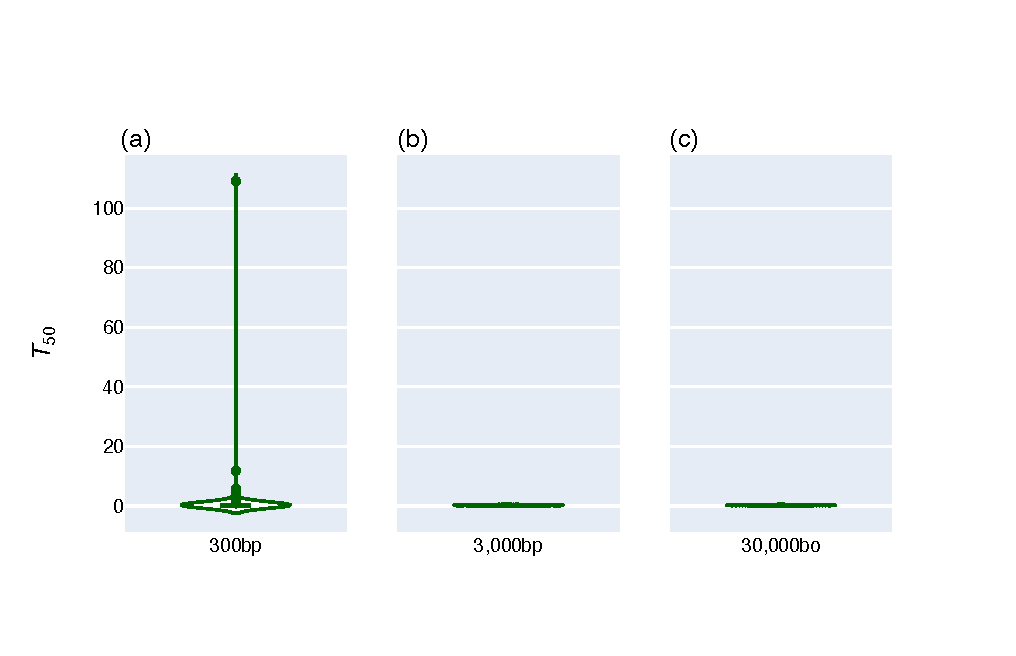
\includegraphics[width=\textwidth]{figures/plots/synthetic/T50/HighJSDLowEntropy-seq_len.pdf}\caption{\textbf{Long Alignments have less sampling error}}
\label{fig:T50-short_long}
\end{figure}

$T_{50}$ estimated under the null was not robust to features of the data. In the simulated stationary data, $T_{50}$ appeared to have a bias towards being highest in the low JSD seeds. The median $\hat T_{50}$ for all simulated data sets is shown in Table \ref{t50_means}. In all but one case, when grouped by length and entropy, the median $\hat T_{50}$ for low JSD $>$ the median $\hat T_{50}$ for high JSD. Recall that JSD is used throughout as a marker of historic disequilibrium. Even though in the simulated data the foreground edge changed to be stationary, it was expected that in the high JSD data sets there would be more disequilibrium in the background edges. It is thus unexpected both that there is a pattern, and that the pattern reflects higher disequilibrium in the low JSD data. This was unexpected and conflicted with the understanding of both $T_{50}$ and JSD.  As a consequence, I did not continue to use $T_{50}$ and you will not see it in further results.

\begin{table}[htbp]
\begin{tabularx}{\textwidth}{ 
  | >{\centering\arraybackslash}X
  | >{\centering\arraybackslash}X 
  | >{\centering\arraybackslash}X 
  | >{\centering\arraybackslash}X  
  | >{\centering\arraybackslash}X | }
\hline  
\textbf{Alignment Length} &\textbf{ High JSD, Low Entropy} & \textbf{ Low JSD, Low Entropy} & \textbf{High JSD, High Entropy} & \textbf{Low JSD, High Entropy} \\
\hline 
    \textbf{300bp} & 0.3184 & 0.3363 & 0.3497 & 0.4576 \\
    \textbf{3,000bp} & 0.2663 & 0.2563 & 0.3096 & 0.3990 \\
   \textbf{30,000bp} & 0.2514 & 0.2778 & .3107 & 0.3911 \\ 
\hline 
\end{tabularx}
\caption{\textbf{Median $\hat T_{50}$ for simulated stationary data sets.} In all but one case, when grouped by length and entropy, the median $\hat T_{50}$ for low JSD exceeded the median $\hat T_{50}$ for high JSD. Each data set contained 1,000 synthetic stationary alignments.}
\label{t50_means}

\end{table}


\subsubsection*{Both tests of equivalence of process were consistent with asymptotic approximations}

A test of equivalence of process can be applied to two comparison, adjacent and temporal. Adjacent is the test of equivalence between neighbouring alignments of the same edge and temporal is the test between one-to-one orthologs. This is a hypothesis test for whether the process is shown to be different: analysing the concatenated alignments is the null (the process is the same); analysing them separately is the alternate (the process is different). Both tests are a comparison of likelihoods between fitting both alignments with one $\mathrm{Q}$ (null), or fitting a separate $\mathrm{Q}$ per alignment (alternate). Significance is assessed with a likelihood ratio, which again, it is necessary to determine whether asymptotic approximations apply. 

The null distribution of the adjacent equivalence of the process test was determined using pairs of synthetic alignments. The simulated data sets are collections of alignments that were generated from the same stationary process. By definition the generating process is equivalent, so any differences in model fits represents sampling error arising from finite data. Since the alignments were generated randomly, I constructed an artificial genome by arbitrarily ordering sequences and then performed a `a sliding window` of size two to select pairs of alignments.

The null hypothesis for the temporal equivalence of process test is that the foreground edges are generated by the same process. This the not the case for the previously mentioned simulated data. To specify the null distribution I again used the four stationary seed alignments, but defined the two foreground edges have the same generating parameters. I simulated data sets of corresponding length to the previously described synthetic data sets. 

Applying both tests to their respective null distributions indicated that they are both consistent with theoretical expectations, presented in Figure \ref{fig:synthetic/adj-temp_eop/HighJSDHighEntropy}. This is illustrated by Quantile-Quantile plots comparing the distribution of p-values to the uniform distribution for the temporal test (fig. \ref{fig:synthetic/adj-temp_eop/HighJSDHighEntropy}a) and the adjacent test (fig. \ref{fig:synthetic/adj-temp_eop/HighJSDHighEntropy}b). The orange line falls very close to the diagonal, demonstrating that the distribution of $\hat p-$values is almost indistinguishable from the uniform distribution.  This result identifies that in application of this test, it is suitable to assume the statistic is $\chi^2_{df}$ distributed and in turn, obtain the $p-$value from analytical distribution. Alignments of length 300 generated by the High JSD, High Entropy seed are shown, however, this result was the same for all seeds and all lengths, included in the appendix (see Fig. \ref{fig:synthetic/adj_eop/all_seeds} and \ref{fig:synthetic/temp_eop/all_seeds}).

\begin{figure}[htbp]
\centering
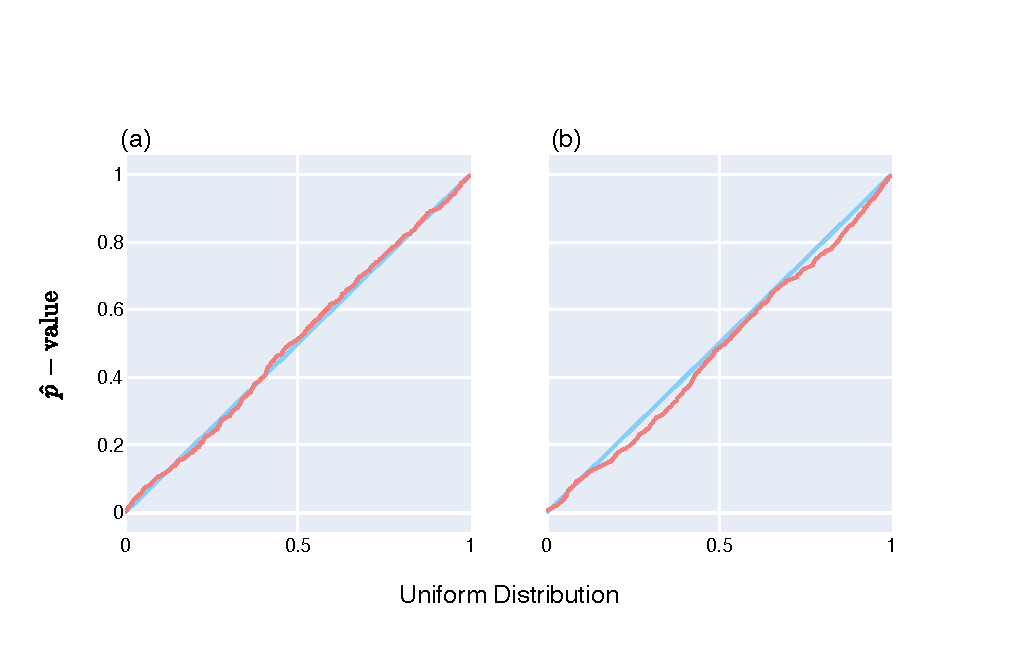
\includegraphics[width=\textwidth]{figures/plots/synthetic/adj-temp_eop/High JSD, High Entropy.pdf}
\caption{\textbf{Both equivalence of process tests were consistent with theoretical approximations.} The Quantile-Quantile plots compare the distribution of $\hat p-$values to the uniform distribution. As the data points (shown as the orange line) fall very close to the diagonal, this demonstrates that the distribution of $\hat p-$values is almost indistinguishable from the uniform distribution. (a) $\hat p-$values from temporal equivalence of process, (b) $\hat p-$values from adjacent equivalence of process. This result is shown for alignments of length 300 generated by the High JSD, High Entropy seed, however, the result was the same for all seeds and all lengths, shown in the appendix, see figure \ref{fig:synthetic/adj_eop/all_seeds} and \ref{fig:synthetic/temp_eop/all_seeds}.}
\label{fig:synthetic/adj-temp_eop/HighJSDHighEntropy}
\end{figure}

\section{Testing the known}

Having lost major components of the DNA methylation process that remain in its sister taxa, the \textit{D. melanogaster} genome is a very useful natural experiment. DNA methylation is a well known mutagenic force. Consequently, the lack thereof in
\textit{D. melanogaster} led to the strong prediction that the \textit{D. melanogaster} genome would exhibit globally high levels of mutation disequilibrium. Because it is a sister taxa to \textit{D. melanogaster} that still methylates its DNA, \textit{D. simulans} provided a necessary point of comparison. I performed two separate analyses, each with either \textit{D. melanogaster} or \textit{D. simulans} as the foreground, and another close taxa that retains methylation, \textit{D. yakubra}, as the outgroup. The analyses were performed on the same alignments of third codon positions from orthologous protein coding genes. The aim was to determine whether the developed methods would reflect the expected form of mutation disequilibrium. The expectations were that the \textit{D. melanogaster} genome would exhibit higher levels of both existence and magnitude of mutation disequilibrium than \textit{D. simulans} and that this would be a genome wide relationship. 

The relative levels of purifying natural selection operating on the chromosomes allows for predictions of the magnitude of mutation disequilibrium in the chromosomes. For hetero-gametic sexes, you expect the chromosome that is hemizygous to be subjected to more stringent natural selection, because any recessive deleterious gene is exposed in the homozygous sex. The prediction is that with the increased magnitude of purifying selection, the rate of convergence to equilibrium should be slower. A slower rate of convergence to equilibrium leads to a higher magnitude of disequilibrium. Therefore, a further expectation was that the X chromosome would exhibit a higher magnitude of mutation disequilibrium relative to the autosomes. 

\subsubsection*{The entire \textit{D. melanogaster} genome is systematically elevated in both the existence and magnitude of mutation disequilibrium compared to its sister taxa, \textit{D. simulans}}

There is a striking elevation of the existence of mutation disequilibrium in the \textit{D. melanogaster} genome when compared to that of \textit{D. simulans}, shown in Figure \ref{fig:drosophila_lrt_qq}. Each subplot in Figure \ref{fig:drosophila_lrt_qq} shows for the observed data, as well as simulated +ve and -ve controls, the distribution of $\hat p-$ values from the test of existence compared to the uniform distribution. The controls are two synthetic cases of ground truth no disequilibrium (-ve), and ground truth there is disequilibrium (+ve). The observed data points of \textit{D. melanogaster}, shown in Figure \ref{fig:drosophila_lrt_qq}b, fall substantially further from the -ve control than that of \textit{D. simulans}, shown in \ref{fig:drosophila_lrt_qq}a. This indicates that, as specified by the test of existence, a much larger proportion of the \textit{D. melanogaster} genome is in mutation disequilibrium than \textit{D. simulans}. The specific proportion of each genome, requires correcting for multiple tests of the same hypothesis. 

\begin{figure}[h]
\centering
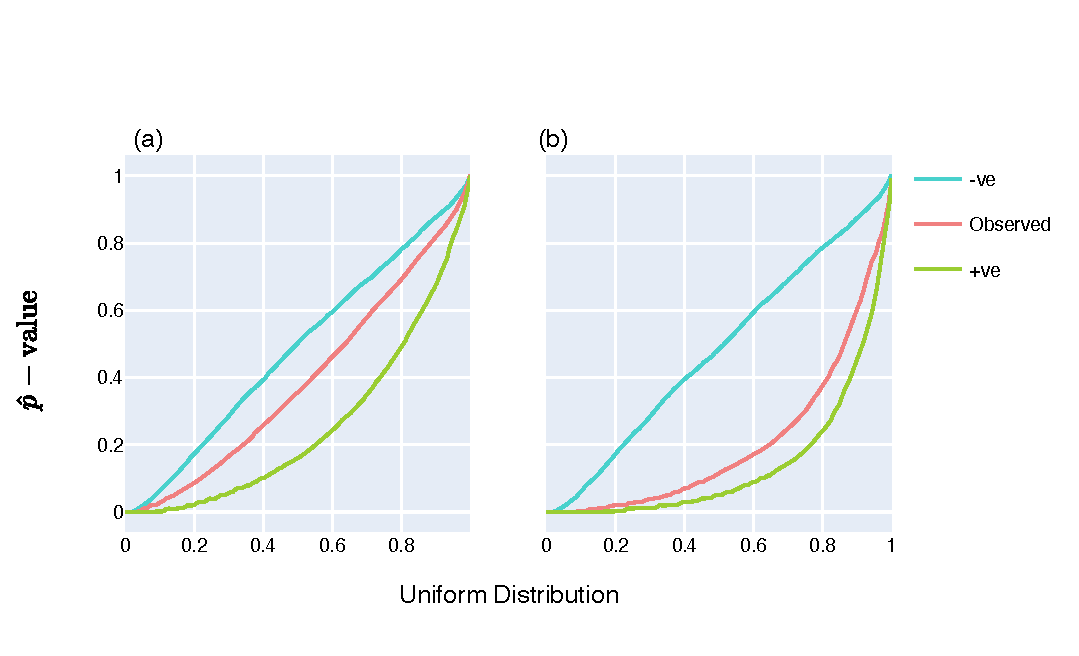
\includegraphics[width=	\textwidth]{figures/plots/drosophila/LRT-QQ.pdf}
\caption{}
\label{fig:drosophila_lrt_qq}
\end{figure}


The resolution of the test of existence $\hat p-$ values is too low for conventional methods of multiple test corrections. The simulation results revealed that under the theoretical distribution the $\hat p-$ values are not uniformly distributed. As a result, they are unsuitable for assessing significance. A method for assessing significance, in this case, is with a parametric bootstrap. The compute time for a bootstrap with a single replicate is ${\sim} 6$ seconds. For each of the Fly data sets there are ${\sim} 4,500$ alignments. In order to satisfy the Bonferroni correction for $4,500$ alignments you would need to, with some level of precision, be able to estimate $p$ values below the altered significance threshold, $0.05/4,500 = 1.1{\times}10^{-5}$. For it to be possible to reject the null requires generating greater than $1/1.1{\times}10^{-5}$ replicates per alignment. This would take $9,009$ hours per alignment, of which there are $>9,000$. This is a prohibitive level of computation that is both impractical, and unnecessary. 

I have established an alternate strategy that takes advantage of the shape of the distribution. The challenge of correcting for multiple tests is pronounced in the space of genomics, for which \cite{Storey2003StatisticalStudies} introduced a formal procedure for estimating the false discovery rate. In their case, they produce an alternate statistic to be interpreted for an individual result, which isn't applicable here due to the low resolution of $p-$values. However, their procedure included an estimation of the fraction of an analysis which is consistent with the null hypothesis. This method takes advantage of how the $p-$values of data that is consistent with the null will be uniformly distributed, illustrated in Figure 1 of \citep{Storey2003StatisticalStudies}. Fitting a cubic spline to determine the inflection point, one can estimate the proportion of a given distribution that is uniform consistent with the null hypothesis, denoted here as $f$. Of interest to this analysis is $1 - f$, the proportion that is not consistent with the null hypothesis. The code to produce $f$ is included in the \href{https://github.com/StoreyLab/qvalue}{qvalue} R package \citep{Storey2004StrongApproach}.

A significantly higher proportion of the \textit{D. melanogaster} genome was estimated to be in mutation disequilibrium compared to \textit{D. simulans}. The estimated proportion ($1 - f$) of the \textit{D. melanogaster} genome which is in mutation disequilibrium is 90\% compared to 50\% of the \textit{D. simulans} genome. Such a substantial difference is a compelling result. Where there is strong evidence of the recent evolution of mutation, \textit{D. melanogaster}, the vast majority of genes are in mutation disequilibrium. In a closely related species where the state of mutation has not so drastically changed, \textit{D. simulans}, only half of the genes are in mutation disequilibrium. This result supports the prediction that the existence of mutation disequilibrium would be elevated in \textit{D. melanogaster} relative to its sister taxa.

The magnitude of mutation disequilibrium, as measured by the $\delta_\nabla$  statistic, is also higher in \textit{D. melanogaster}. Figure \ref{fig:drosophila_d-conv-diff} shows a direct comparison allowed by the paired nature of the data sets. Each data point in Figure \ref{fig:drosophila_d-conv-diff} is the difference between $\hat \delta_\nabla$ for a \textit{D. melanogaster} gene and its ortholog in \textit{D. simulans}. These are genes with essentially the same function, but evolving under presumably different mutagenic environments. The distribution in Figure \ref{fig:drosophila_d-conv-diff} is right shifted, showing that most genes have a higher $\delta_\nabla$ estimate in \textit{D. melanogaster}. This result supports the prediction that the magnitude of mutation disequilibrium would be elevated in \textit{D. melanogaster} relative to its sister taxa. 

\begin{figure}[h]
\centering
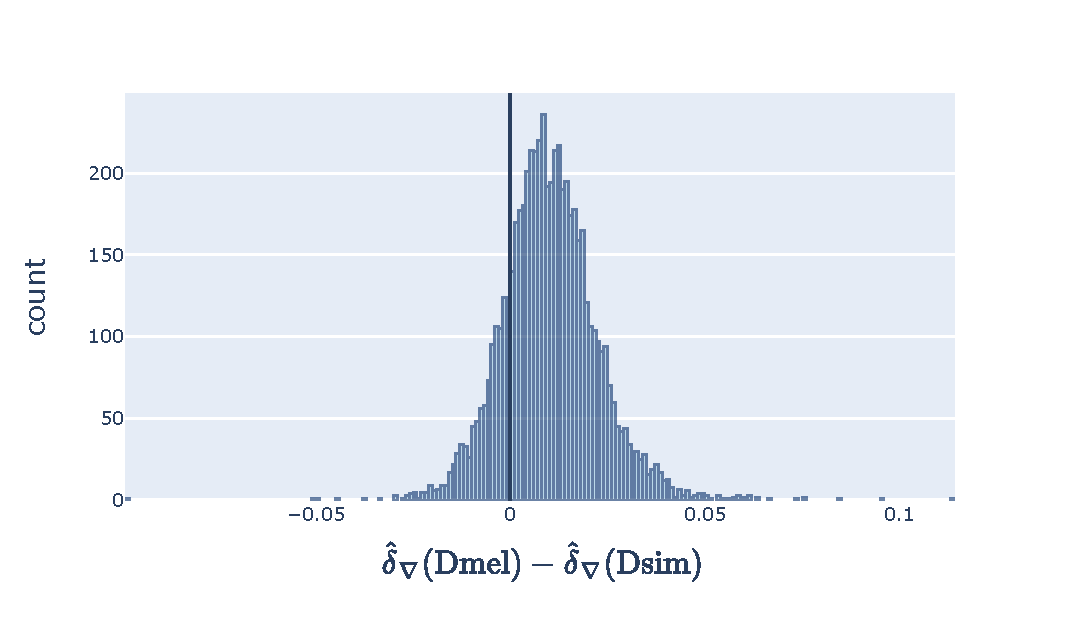
\includegraphics[width=	\textwidth]{figures/plots/drosophila/d-conv-diff.pdf}
\caption{\textbf{The magnitude of mutation disequilibrium is higher in \textit{D. melanogaster} genes.} }
\label{fig:drosophila_d-conv-diff}
\end{figure}


The pattern of elevated mutation disequilibrium is systematic across the \textit{D. melanogaster} genome. The $\hat \delta_\nabla$ for a chromosome is shown with a horizontal line in Figure \ref{fig:drosophila_d-conv_manhattan}, where for all chromosomes analysed, \textit{D. melanogaster} clearly exceeds \textit{D. simulans}. In fact, comparatively, the \textit{D. simulans} genome appears to be centred very close to zero. The consistency of elevation throughout the genome is in accordance with prior predictions.

Strong purifying selection impedes the rate of convergence of the X chromosome. Considering that the X chromosome has fewer data points, it is evident in Figure \ref{fig:drosophila_d-conv-diff} that the \textit{D. melanogaster} X has an larger proportion of high $\hat \delta_\nabla$ than all other chromosomes shown. The median $\hat \delta_\nabla$ for chromosomes 2, 3 and X in \textit{D. melanogaster} is $0.0132$, $0.0131$ and $0.0177$ respectively. The median $\hat \delta_\nabla$ for chromosomes 2, 3 and X in \textit{D. simulans} is $0.0031$, $0.0031$ and $0.0040$ respectively. For both species the X chromosome clearly has a higher median $\hat \delta_\nabla$ than the autosomes, consistent with a slower rate of convergence and thus a higher magnitude of disequilibrium for sequence acted upon by purifying selection. 

\begin{figure}[htbp]
\centering
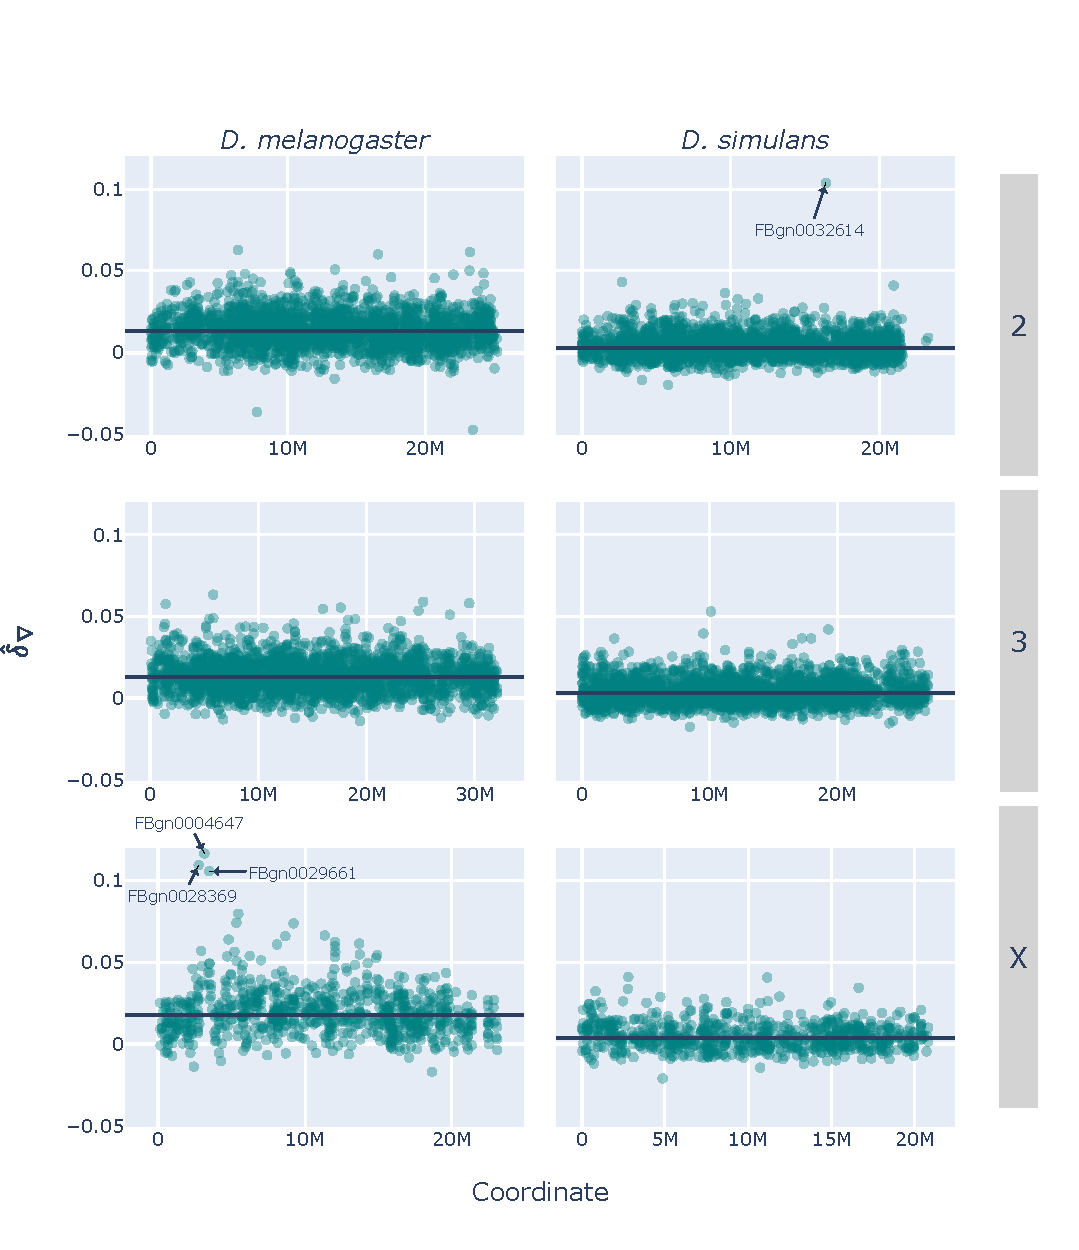
\includegraphics[width=\textwidth]{figures/plots/drosophila/d-conv_manhatten.pdf}
\caption{\textbf{The pattern of elevated mutation disequilibrium in \textit{D. melanogaster} compared to \textit{D. simulans} is systematic across the genome}. Manhattan plots the position of a gene in a chromosome and the $\hat\delta_\nabla$ for the CDS sequence of that gene. The CDS sequence is third codon position only. The median $\hat\delta_\nabla$ is indicated for a chromosome with a horizontal line. The number of genes included in the plots of chromosome 2, 3, and X of \textit{D. melanogaster} is 2373, 2624 and 818 respectively. For chromosome 2, 3, and X of \textit{D. simulans}, the number of genes is 2388, 2623 and 800 respectively.}
\label{fig:drosophila_d-conv_manhattan}
\end{figure}


Link back to the aim and whether the result show what I aimed to show. 

\section{Testing the conjectured}

Recombination and its association with GC-biased gene conversion has been proposed to be a major force in the formation of isochores \citep{Montoya-Burgos2003RecombinationGenomes}. The translocation of \textit{Fxy} in \textit{M. musculus} such that half of the gene now resides in the only recombining part of the X chromosome is a unique natural experiment from which that conjecture may be corroborated. This perturbation is predicted to have led to elevated disequilibrium in the region that has moved into the PAR, relative to the component of the gene that remains in the uniquely X region. To test this prediction I used alignments of \textit{Fxy} in \textit{M. musculus} with orthologs from \textit{M. spretus} and \textit{R. norvegicus}. For all model fitting, \textit{M. musculus} was the foreground edge. I analysed the first six introns of Fxy, of which in \textit{M. musculus} the $5'$ end (exons 1-3) is X-specific, and the $3'$ end (exons 4-6) is located in the PAR. The boundary of the PAR is found in the third intron \citep{Palmer1997AMice}. The evolutionary history of \textit{Fxy} in rodents alongside the structure of \textit{Fxy} in \textit{M. musculus} is shown in Figure \ref{fig:Fxy}. 

I aimed to determine whether the current understanding of how this translocation may affect the divergence process would be reflected by the methods. Because the entire gene had been translocated, I expected the whole gene to be in mutation disequilibrium. Considering the distinct mutagenic properties of the PAR, I aimed to see whether by using the statistic of magnitude, $\delta_\nabla$, I could detect elevated levels of disequilibrium in the PAR-located half. A specific location of the boundary is not provided, therefore, I aimed to see whether the magnitude of mutation disequilibrium locally within intron 3 would illustrate where the boundary is located. 

\begin{figure}[htbp]
\centering
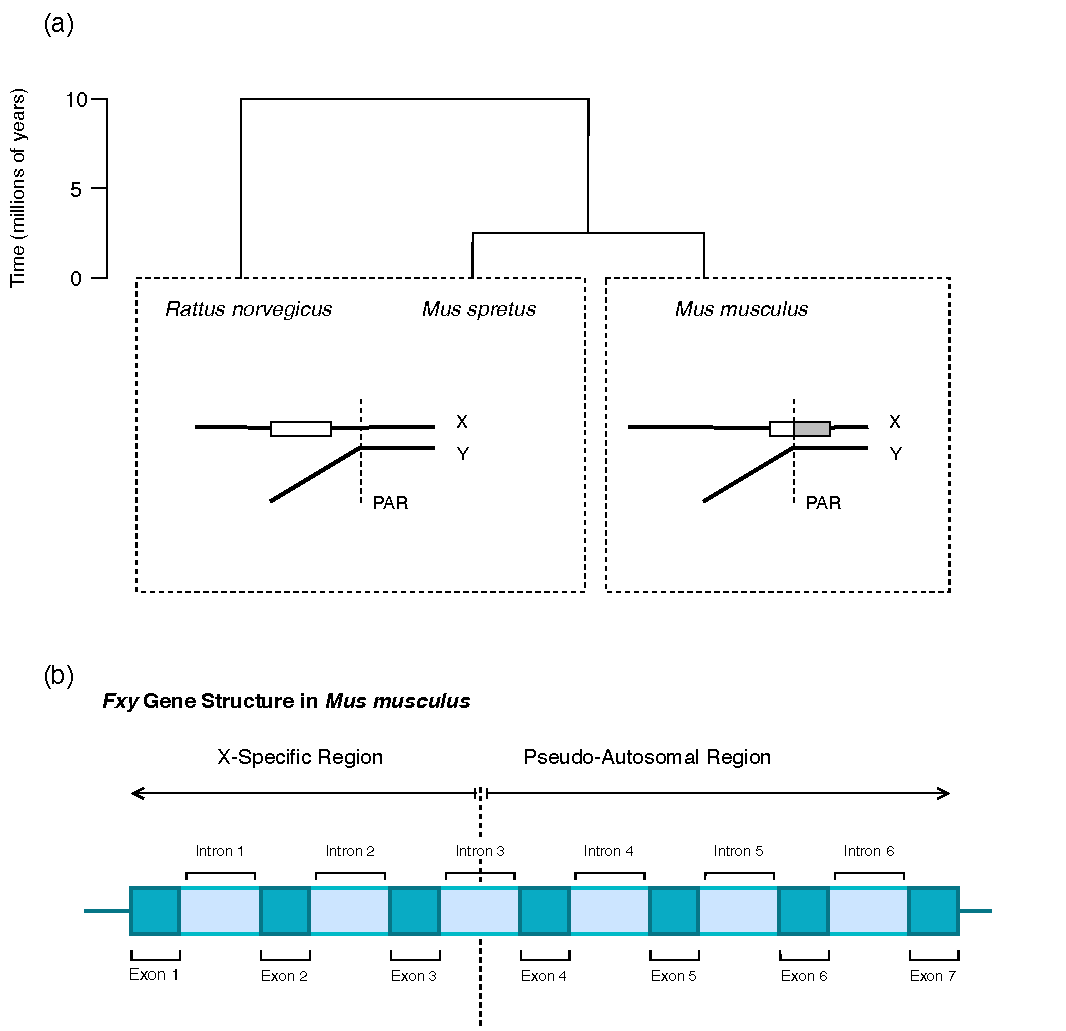
\includegraphics[width=\textwidth]{figures/diagrams/Fxy.pdf}
\caption[Evolutionary History of \textit{Fxy} in Rodents]{\textbf{Evolutionary History of \textit{Fxy} in Rodents}. \textbf{(a)} The \textit{Fxy} gene in \textit{M. musculus} was translocated from a X-specific position to a new position in which it overlaps with the PAR. The overlap in \textit{M. musculus} is shown as the shaded region of the gene, shown as a box. The divergence timescale is indicated in millions of years. In rodents and other mammals \textit{Fxy} is X-specific, suggesting translocation to the PAR in \textit{M. musculus} after divergence with \textit{M. spretus}, between 2-3 million years ago \citep[adapted from Figure 1][]{Galtier2007AdaptationEvolution}. \textbf{(b)} The structure of the \textit{Fxy} gene in \textit{M. musculus}. The $5'$ end of the gene, exons 1-3, are X-specific. The $3'$ end of the gene, exons 4-10, are positioned in the PAR. Note that for simplicity, exons beyond exon 7 are not shown in the structure. The boundary to the PAR falls in intron 3 of \textit{Fxy} \citep{Palmer1997AMice}. }
\label{fig:Fxy}
\end{figure}

\subsubsection{The PAR-half of \textit{Fxy} has elevated mutation disequilibrium relative to the X-linked half in \textit{M. musculus}}

Although the entire \textit{Fxy} gene is in mutation disequilibrium, the magnitude of mutation disequilibrium is substantially higher in the $3`$ end of the gene relative to the $5`$ end. The estimated $\hat p$-value from the test of existence applied to each intron is shown in Table \ref{table:nablaFxy}. With the exception of intron 3 where the $\hat p$-value was $0.01$, all other introns had a $\hat p$-value of $0.00$. This result validates the need to develop methods of quantifying mutation disequilibrium, for with this result alone, the X-specific and PAR-located regions are indistinguishable. However, for the $\delta_\nabla$ statistic, there is a clear difference between the two regions. $\hat \delta_\nabla$ for each intron is shown in Table \ref{table:nablaFxy}, for which the introns in the PAR (4-6) are significantly higher than those that are X-specific (1-2). In fact, the smallest $\hat \delta_\nabla$ in the PAR (intron 5) is still 19 times larger than the largest $\hat \delta_\nabla$ not in the PAR (intron 2).

\begin{table}[htbp]

\begin{center}
\setstretch{1.6}
\begin{tabularx}{\textwidth}[t]{ 
  | >{\centering\arraybackslash}c 
  | >{\centering\arraybackslash}X 
  | >{\centering\arraybackslash}X  
  | >{\centering\arraybackslash}X  
  | >{\centering\arraybackslash}X  
  | >{\centering\arraybackslash}X  
  | >{\centering\arraybackslash}X | 
  }
\hline
\textbf{{Intron Rank}} & \textbf{{1}} & \textbf{{2}} & \textbf{{3}} & \textbf{{4}} & \textbf{{5}} & \textbf{{6}} \\
\hline
ToE $\hat p$-value & 0.00 & 0.00 & 0.01 & 0.00 & 0.00 & 0.00 \\
\hline
$\hat\delta_\nabla$ & 0.0019 & 0.0024 & 0.0115 & 0.0490 & 0.0470 & 0.0671 \\
\hline
\end{tabularx}
\end{center}
\caption{\textbf{The magnitude of mutation disequilibrium is highest in the region of the \textit{Fxy} gene that resides in the PAR.}}
\label{table:nablaFxy}

\end{table}

There is a clear differences in $\hat \delta_\nabla$ either side of intron 3. The portion of the gene $5'$ to intron 3 is X-specific, while the $3'$ portion is located in the PAR. This result motivated a closer analysis of intron 3 to try and identify a "break point" at which the process shifts. To tackle this aim I performed a sliding window $5' \rightarrow 3'$ along the alignment of intron 3, computing $\hat \delta_\nabla$ for each window. The window took $600$ positions of the raw alignment, filtered the alignment and if at least 300 positions remains, computed $\hat \delta_\nabla$. 

Sliding window analysis showed that $\delta_\nabla$ oscillates within intron 3, with the amplitude of the oscillation largest at the $3'$ end, illustrated in Figure \ref{fig:rodent/d-conv/intron3}. For each window, $\hat \delta_\nabla$ is plotted against the location of the window midpoint, noting that the location is with respect to \textit{M. musculus}. The location of annotated repeats in \textit{M. musculus} are shown on the bottom of the figure, of which the different colours simply indicate different classes of repeats. The figure shows a period of oscillation in $\hat \delta_\nabla$ that is considerably consistent across the intron. These local fluctuations meant that the aim of determining a break point could not be so simply met. Remarkably, the local fluctuations still exhibit a marked increase in amplitude towards the $3'$ end of the intron. This is of considerable interest, although the underlying process has repetitive local changes, there is still an identifiable change in the process in the region of the intron expected to be in the PAR. Furthermore, the oscillation appears to be a feature of \textit{Fxy} introns, as all introns exhibited such a pattern (data shown in appendices.)

\begin{figure}[htbp]
\centering
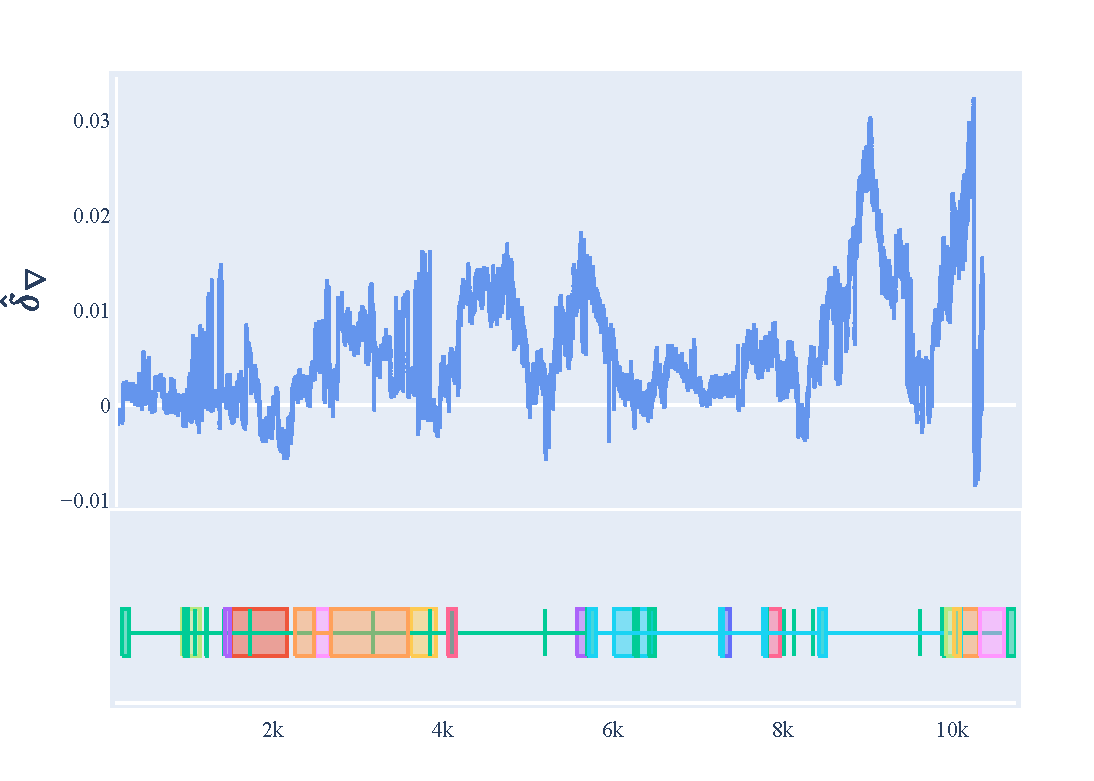
\includegraphics[width=\textwidth]{figures/plots/rodent/dconv-intron3.pdf}
\caption{$\hat\delta_\nabla$.}
\label{fig:rodent/d-conv/intron3}
\end{figure}

The conjectured impact of recombination on the divergence of sequence located within the PAR, is reflected in these developed methods. The results show that although the entire translocated \textit{Fxy} gene rejected the null of mutation equilibrium, the magnitude of disequilibrium was strongest in the half that is now located in the PAR. I uncovered that within the introns there is fascinating pattern of magnitude of disequilibrium, furthermore, the entire pattern is magnified towards the PAR. These results support local rearrangements being a mechanism of mutation disequilibrium and that the more distinct the mutagenic environment in the new location, the higher the magnitude of mutation disequilibrium. Thus, the current understanding of how mutagenesis affects the divergence process is reflected when perturbations happen and there is disequilibrium. Such a positive empirical control adds strength to the confidence in the developed measures and their effective detection and measurements of mutation disequilibrium. 

\section{Testing the unknown}

The question of whether the human genome is at mutation equilibrium is of interest to most humans. Unlike the previous two empirical applications, there is no obvious mechanism providing and expectation for the level of mutation disequilibrium. But it is because of the effectiveness of the methods in the previous empirical applications that there are grounds for interpreting the results without such a clear mechanism. I aimed to test for the existence and measure the magnitude of mutation disequilibrium in the human genome. To this end I used  intronic and CDS sequence alignments of chromosome 1 of human, chimpanzee and gorilla. 

\subsubsection{The majority of the human genome is in mutation disequilibrium}


\begin{figure}[h]
\centering
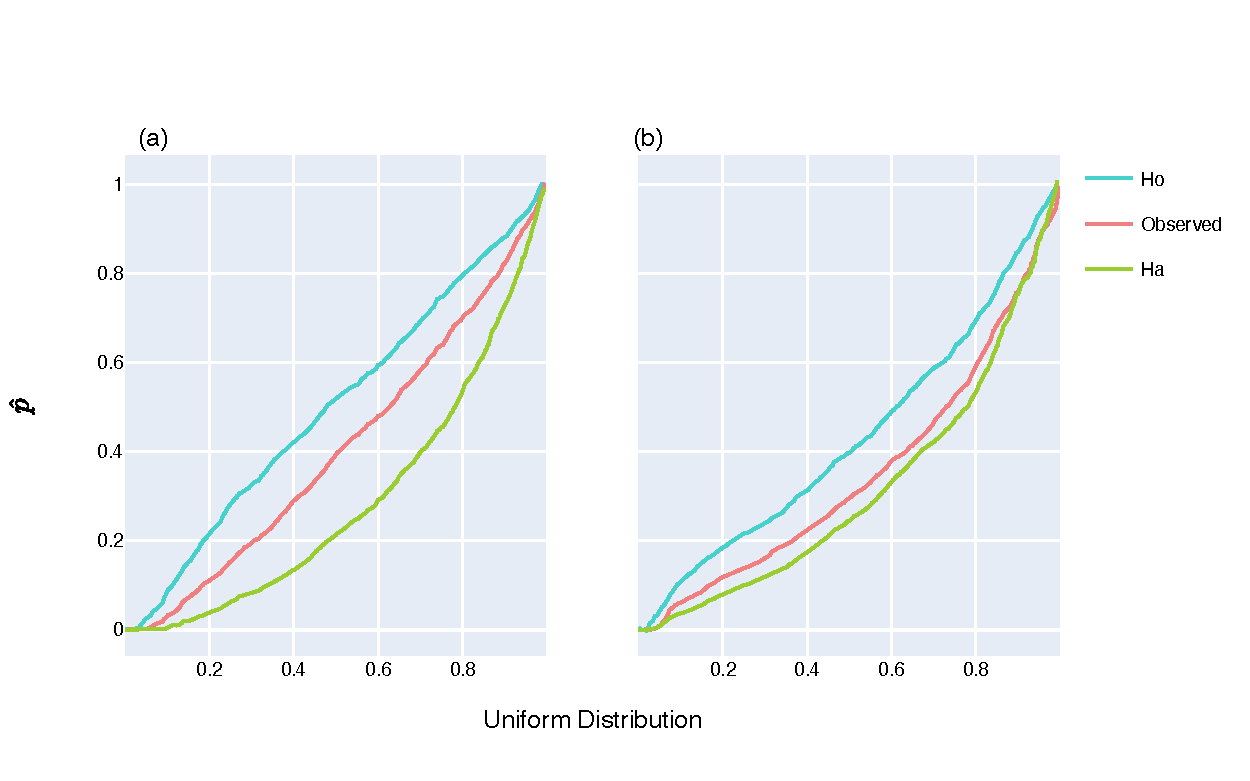
\includegraphics[width=	\textwidth]{figures/plots/primate/LRT-QQ.pdf}
\caption[Humans exhibit a higher proportion of mutation disequilibrium in CDS compared to introns]{\textbf{Humans exhibit a higher proportion of mutation disequilibrium in CDS compared to introns.} The Quantile-Quantile plots compare the distribution of $\hat p-$values to the expected uniform distribution. \textbf{(a)} 1,406 alignments of introns from human, chimpanzee and gorilla, \textbf{(b)}, 1,182 CDS alignments from human, chimpanzee and gorilla. For all model fitting human was the foreground edge. }
\label{fig:primate_lrt_qq}
\end{figure}



\subsubsection{Purifying natural selection impedes the rate of convergence}

\begin{figure}[h]
\centering
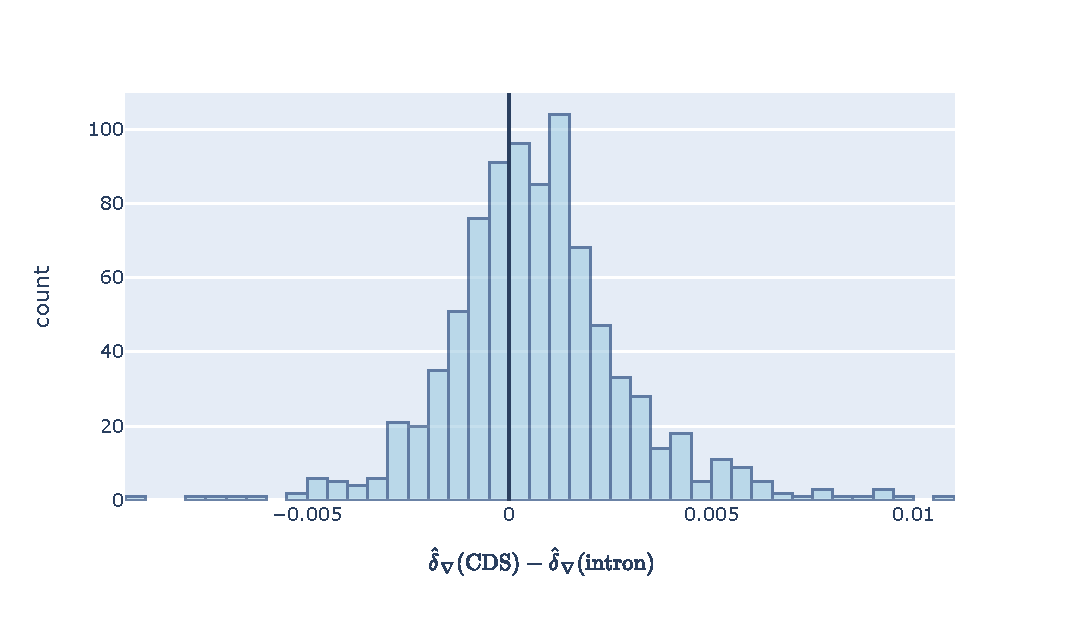
\includegraphics[width=	\textwidth]{figures/plots/primate/d-conv-diff.pdf}
\caption{}
\label{fig:primate:dconv-diff}
\end{figure}


\chapter{Discussion}

Disequilibrium of mutagenesis is a phenomenon that is widely assumed not to exist, almost never examined, but potentially of profound significance with likely important applications. In this work, I have addressed the development of statistical methods of testing for its existence and characterising the form that it takes. I have found: it exists; is greater in magnitude following perturbations on local and global scales; and differs between samples. I unified simulation study and empirical knowns, allowing the application to an unknown case, in which I demonstrated that even over short time frames for relatively closely related species, more than half of the human genome is not a equilibrium. The basis for those conclusions and their implications will be discussed below. 

Before launching into a full discussion of this work, I will enumerate a few underpinning assumptions. I assume that the given sequence data is an accurate depiction of the true DNA sequence, and that both annotation of orthology and the alignment path are correct. These are standard assumptions. I have performed both automated (ref) and manual (ref) quality control checks on the alignments. I do not imagine this has eliminated all errors, however, understanding the impact of these assumptions is not addressed in this thesis. 

\section{Outcomes of the unified statistical development process}

\subsection{Lessons from simulations under the null}
The simulation study evaluated the proposed methods on corner cases of the null hypothesis. This was a foundational step, in which I characterised the methods in known environments. The simulations provided valuable outcomes of how to perform the analyses, and equally importantly, when not to. 

A major outcome of the simulation study was identifying the paradoxical behaviour of the $T_{50}$ statistic. Theoretically, $T_{50}$ is a natural measure. It uses biologically interpretable units in a way conceptually related to measures employed in other disciplines. It appears, however, that a half-life statistic does not work for this type of stochastic process (Section \ref{T50_results}). Although I interrogated a number of things I thought might be the cause, that line of inquiry is incomplete. At this point, it is not entirely certain what is the problem, but it does not appear to be a fruitful measurement for future research. 

One imaginable explanation of the failings of $T_{50}$ is in its implicit assumption of the relationship between substitution events and chronological time. Consider the following thought experiment. The decay of non-stationarity is exponential. When you are far from equilibrium, many of the substitutions will take you closer to equilibrium. When you are really close to equilibrium, more of the substitutions will look like noise, and take you away from equilibrium. The halfway point is defined in terms of changes in the composition. So, perhaps in the asymptotic tail, halfway can be further away. Although just a thought experiment, this paradox demonstrates that it is not obvious how to choose a metric, and your intuition is not always correct. 

The outcome for the $\delta_\nabla$ statistic was quite the opposite. The strong relationship between $\delta_\nabla$ and historical disequilibrium was very encouraging, as it supported that $\delta_\nabla$ is in fact measuring what it is intended to measure, mutation disequilibrium (Section \ref{nabla_results}).

The simulation study identified the appropriate basis for conducting the hypothesis tests. This step identified where the asymptotic assumptions do not hold, a crucial discovery for the TOE (Section \ref{TOE_results}). As conventional asymptotic approximations to the TOE distribution were shown not to hold, $p$-values were estimated via parametric bootstrap. As a result, the TOE is a robust test for the existence of mutation disequilibrium, allowing for confidence in application to natural data. 

\subsection{Does mutation disequilibrium exist?}

\subsubsection{High levels of mutation disequilibrium in \textit{D. melanogaster} mirrors recent loss of methylation}
I tackled the known cases of testing for mutation disequilibrium in \textit{D. melanogaster} and its sister taxa, \textit{D. simulans}. Using the TOE, I estimated that the proportion of genes that were in mutation disequilibrium was 90\% and 50\% for \textit{D. melanogaster} and \textit{D. simulans} respectively (Section \ref{TOE_drosophila}).  The simulans lineage had previously been shown to have a much higher level of disequilibrium, estimated by \cite{Squartini2008QuantifyingProcess} to be over 85\%. 

The discrepancy with previous disequilibrium estimates is because of the mistaken assumption of the asymptotic distribution by \cite{Squartini2008QuantifyingProcess}. When I applied the test statistic of \cite{Squartini2008QuantifyingProcess} to the data simulated under the null, it was abundantly clear that it does not satisfy the asymptotic distribution (Figure \ref{fig:synthetic/chi2/all-seeds}). Consequently, they excessively rejected the null hypothesis, ultimately causing their estimate to be incorrect.

The higher level of mutation disequilibrium in \textit{D. melanogaster} relative to \textit{D. simulans} supports the hypothesised impact of losing $^5$mC. In comparison to non-methylated cytosine, $^5$mC is hypermutable, with higher rates of deamination to thymine \citep{Shen1994TheDNA, Coulondre1978MolecularColi}. If not correctly repaired, what was originally a G-C pairing turns into a A-T pairing. The loss of $^5$mC in \textit{D. melanogaster} would remove this mutational bias towards creating A-T pairings. Hypothetically, any equilibrium that had been achieved with $^5$mC present may no longer constitute and equilibrium with respect to the mutagenic process without it. Indeed, 90\% of \textit{D. melanogaster} is not in equilibrium (Section \ref{TOE_drosophila}). Such a substantial difference is a compelling result. Where there is strong evidence of the recent loss of $^5$mC, the vast majority of genes are in mutation disequilibrium. In a closely related species where the state of mutation has not so drastically changed, only half of the genes are in mutation disequilibrium.

The substantive difference in disequilibrium between the species is clear, however, the conjectured cause was not directly interrogated. It is possible to support the interpretation in other ways, because the mechanism has other predictions that can be verified. The hypermutability of $^5$mC creates a mutational bias towards creating A-T base pairings. A simple supplementary analysis would look at whether the equilibrium nucleotide distribution of \textit{D. melanogaster} is then increasing in terms of GC content. 

To directly interrogate the impact made by the presence or absence of $^5$mC would require implementing a dinucleotide model. $^5$mC primarily affects cytosine found in CpG dinucleotides, consequently depleting such dinucleotides from the genome \citep{Holliday1975DNADevelopment, Bird1980DNADNA}. To extend my methods to account for this process requires the combination of a few approaches. To take into account the impact of $^5$mC requires an approach presented in \cite{Huttley2004ModelingMammals}, of adding a parameter specifically for the mutation of CpG. Additionally, as it is modelling protein coding sequence, it is critical to deal with the confounder of natural selection operating on non-synonymous changes. This is achieved by the General Nucleotide Codon (GNC) model \citep{Kaehler2017StandardData}. Mapping a CpG parameter in into the GNC model would achieve the goal, however, it is important to note that the large number of free parameters would make any application exceedingly slow. Generalising my statistics for application to a dinucleotide process is an important avenue for future development. 

Modelling evolution as an independent nucleotide process is a fundamental limitation of my methods and consequently a caveat to all my results. As illustrated above, the mutation process does not act on single nucleotide. In fact, it appears that the mutagenesis is substantially affected by the context of neighbouring bases \citep{Zhu2020MachineMutations}. Known as Simpson's Paradox \citep{Simpson1951TheTables}, it is possible that the increased mutation disequilibrium in \textit{D. melanogaster} relative to \textit{D. simulans}, along with all other results, are limited to the nucleotide dimension and would not appear in an analysis in another dimension (e.g., a  dinucleotide process). On the other hand, it is also possible that the result could be more pronounced. To that end, I defer to the words of George Box,``All models are wrong, some are useful''. 

I tested for the existence of mutation disequilibrium in the recently translocated \textit{Fxy} gene in \textit{M. musculus}. I aimed to see if section of the gene located in the PAR would be further from equilibrium than the X-specific section. Applying the TOE to the first six introns, I determined that all introns analysed were in mutation disequilibrium (Section \ref{Fxy_TOE}). This result validated the need to develop methods of quantifying mutation disequilibrium, for with this result alone, the X-specific and PAR-located regions were indistinguishable.

\subsection{What is the magnitude of mutation disequilibrium?}

A significant outcome of this thesis is the development of the novel statistic $\delta_\nabla$, a measure of the magnitude of mutation disequilibrium (Section \ref{nabla}). The effectiveness of $\delta_\nabla$ was shown by its capacity to detect predicted elevation of mutation disequilibrium following perturbations. I will discuss the application of $\delta_\nabla$ to positive empirical controls below.  

\subsubsection{The magnitude of mutation disequilibrium is higher following local changes in the mutagenic environment}

Applying $\delta_\nabla$ to \textit{Fxy} clearly separated the X-specific and PAR-located regions (Section \ref{Fxy_TOE}). The region of the gene which is located in the PAR exhibits a markedly higher magnitude of disequilibrium than the X-specific region. Due to the higher levels of meiotic recombination in the PAR, it is natural to consider recombination as a likely cause. 

Recombination is thought to affect the evolutionary process in three ways \citep{Galtier2004RecombinationParadox}. 

There is substantial evidence that recombination is a driving force of GC rich regions of genomes \citep{Meunier2004RecombinationGenome, Berglund2009HotspotsGenes,Galtier2009GC-biasedPrimates}. The conjectured mechanism is biased-gene conversion (BGC), where GC-alleles have a higher probability of fixation than AT-alleles \citep{Eyre-Walker1999EvidenceDNA., Mancera2008High-resolutionYeast}. This mechanism is supported by the results of \cite{Montoya-Burgos2003RecombinationGenomes}, who found that the section of \textit{Fxy} in the PAR exhibited a substantial increase in GC content.

Alternate explanations of this local increase in mutation disequilibrium are not as compelling. It is possible that this result is due to another distinct feature of the PAR, homology with the Y chromosome. The X-linked PAR recombines with the Y-linked sequence, which is further subjected to the higher germ-line mutation rate of males \citep{Huttley2000HowMutagenesis}. As male mutational bias does not appear to be linked to increased GC content, this explanation is less probable. 

\subsubsection{The magnitude of mutation disequilibrium is higher following global changes to mutation}

To measure the magnitude of mutation disequilibrium on a global scale I applied $\delta_\nabla$ to \textit{D. melanogaster} and \textit{D. simulans} genomes (Section \ref{TOE_drosophila}). The mean of $\delta_\nabla$ was significantly higher in \textit{D. melanogaster} relative to \textit{D. simulans}, consistent across all chromosomes. In fact, $82$\% of genes had a higher magnitude of mutation disequilibrium in \textit{D. melanogaster}. Following an event that has caused disequilibrium, as the process approaches equilibrium, $\delta_\nabla$ will asymptote to zero. Therefore, the level of $\delta_\nabla$ in \textit{D. melanogaster} indicates that disequilibrium has been recently created. It is a reasonable hypothesis that the loss of $^5$mC is the driving force behind this elevated disequilibrium, however, it is difficult to rule out other factors. 

An intrinsic limitation of analysing historical processes is that the $\delta_\nabla$ statistic cannot determine or distinguish between causes. Considering that the methylation of DNA has a key role in the epigenetic regulation of gene expression \citep{Holliday1975DNADevelopment, Compere1981DNACells, Lieberman1983UltravioletDemethylation}. Furthermore, in mammalian embryos, the loss of methylation is lethal \citep{Panning1996DNAGenes}. Such is pure speculation, however, \textit{D. melanogaster} presumably has another method of regulating gene expression in lieu of methylation. If such a mechanism exists and has evolved recently, it may be contributing to the marked increase in mutation disequilibrium. 

Principal Component analysis. 

\subsubsection{The magnitude of mutation disequilibrium is variable within an intron}

The oscillation of $\delta_\nabla$ within introns may be caused by the unique chromatin structure of the PAR. 

How to confirm this association

How to test this hypothesis. 




\subsection{Does mutation disequilibrium differ between samples?}

I developed two EOP tests to tackle the statistical problem of whether two related sequences were evolving by an equivalent process. The EOP tests are crucial components of the contribution of my methods to biology. 

\subsubsection{The process was shown to be similar between \textit{D. melanogaster} and \textit{D. simulans} }

The process of mutation was shown to be overwhelmingly similar between orthologs of \textit{D. melanogaster} and \textit{D. simulans}, with only 5\% of genes rejecting the null of equivalence (Section \ref{TOE_drosophila}). Considering the substantially different levels of mutation disequilibrium existence and magnitude between the species, and the fact that one species is methylating and the other is not, this was an unexpected result. 

Assuming that the genes are evolving by the same process, a natural first question to ask is whether the simulans lineage is simply evolving faster and thus is closer to equilibrium already. If this was the case, then we would expect for most genes that the branch length of the \textit{D. simulans} edge would be greater. However, we actually see the opposite, (Figure \ref{fig:drosophila_d-conv-diff}a) and for 75\% of genes, the \textit{D. melanogaster} ortholog has a longer branch length, making this explanation unlikely. 

Simpson's paradox may help explain the disagreement between levels of existence and equivalence of mutation disequilibrium in \textit{D. melanogaster} compared to \textit{D. simulans}. As explained above, the hypothesised mechanism of disequilibrium, $^5$mC, is more appropriately modelled as a dinucleotide process. Perhaps, two processes that are not discernible on a nucleotide level, may be radically different on the dinucleotide level. Again, to determine if this is the case would require implementing the methods as a dinucleotide process. 

How come the difference was determined by the TOE and the magnitude statistic?

The power of the test may also influence this result. It is also possible that the temporal Equivalence of Process is simply a low powered test. This may result from the choice to model all edges as continuous time. 

I therefore conclude that the most likely explanation for these results is a combination between the low power of the test and the fact that the change in the process has occurred on a dinucleotide level. 

\subsubsection{There are significantly different evolutionary processes within the \textit{Fxy} gene}

I tested whether adjacent \textit{Fxy} introns were evolving by an equivalent process. I found that the introns within the PAR were evolving by the same process, yet all other adjacent comparisons were evolving by different processes (Section \ref{Fxy_TOE}). 

It is tempting to imagine that this result reflects the historical inclusion of these sequences in the PAR. The addition/attrition hypothesis of evolution of the sex chromosome proposes that genetic material is added to the PAR and is initially present on both the X and Y chromosomes, but is followed by attrition of the pseudoautosomal sequence on the Y chromosome  \citep{Graves1995TheGenes}. Perhaps we are seeing the influence of the amount of time each intron spent in the PAR. 

The time frame of the translocation of \textit{Fxy} makes this hypothesis practically infeasible. The boundary of the PAR in humans is estimated to have shifted a mere 240bp due to attrition since divergence with other great apes, approximately 19MYA \citep{Mensah2014PseudoautosomalPopulation}. This makes the attrition of greater than 120,000bp of the \textit{M. musculus} Y chromosome in the 2-3 million years (MY) since divergence with \textit{M. spretus} extremely unlikely \citep{Huang2005HowMammals}. 

Ultimately, this result appears to be confounded by the length of the introns. The X-specific introns have a mean length of $\sim28,000$, an order of magnitude larger than the PAR located introns, which have a mean length of $\sim2,300$. The power of a hypothesis test is the probability of the test correcting rejecting the null hypothesis. The power of the EOP test is affected by the number of substitution events that distinguish the sequences in an alignment. A longer alignment is more likely to have more substitution events and thus increase the power of the test. Therefore, it seems most likely that this result simply reflects the relative power of each test, in turn, the length of the alignments. 

\section{Is the Human genome at equilibrium?}

I now turn my attention to the evolution of the human genome. Unlike the application to empirical controls, there was no expectation of the level or form of mutation disequilibrium. 

\subsubsection{There is substantial evidence for the existence of disequilibrium in the human genome}

I estimated the proportion of the chromosome which was in disequilibrium to be $\sim50\%$ for intronic sequence and $\sim68\%$ for CDS (Section \ref{Human:TOE}). Acknowledging Simpson's paradox, these results strongly suggest the existence of disequilibrium in more than half of the examined sequences. What these results do not guarantee is that that the disequilibrium is a consequence entirely of changes to mutagenesis. In fact, for the CDS result, I expect that the level of disequilibrium is influenced by selection. However, I can potentially rule it out as a major factor in the intronic sequences. 

The determination that selection is operating is often based on variability and rates of evolution (ref). The underlying premise of that work is often that the neutral rate is uniform (ref). The challenge to that is the strong evidence that mutagenesis is not uniform (ref). As a consequence, those conclusions are in doubt, until we have a clearer understanding of what the true baseline of neutral processes look like. What this means is not that everything is neutral, just that until demonstrated otherwise, we cannot establish whether it is neutral or adaptive. 

It seems more likely that most genomic sequence, even within introns or between genes, is not functional. The demonstrated abundance of functional elements outside of protein coding sequences is low \citep{Graur2013OnENCODE} and the average length of protein binding motifs is approximately 10nt \citep{Stewart2012WhyLong}, a minor proportion of the typical length of an intron, $\sim7,000$bp \citep{10.1093/database/baw153}. These observations are not definitive, but they argue against the abundance of natural selection being the force behind these transitions. 

In light of the previous arguments, it is plausible that the level of disequilibrium in the intronic sequences is largely due to changes to mutagenesis. 

The estimate of the proportion of the CDS data in disequilibrium may be imprecise due to underlying differences between each gene. An assumption of the approach of \cite{Storey2003StatisticalStudies} is that each data point is a result from data drawn from the same underlying distribution, in which case, you can expect that the $p$-values are uniformly distributed. When you are not drawing randomly from the same distribution, even when the null is true, that expectation is not met. This is the case for the CDS analysis, where the data generated under the null hypothesis does not fall on the diagonal line (Figure \ref{Human:TOE}), illustrating the impact of differences such as the length of alignment or rate of evolution. The properties of the estimate are not entirely understood as a consequence, however, the departure from theory is small enough that there is still something to be gained from this data. There is this way to determine what the correct proportion is. This would be to randomly draw from the true negative and true positives in different proportions and try to solve for the observed fraction. 

\subsubsection{The magnitude of disequilibrium is heterogeneous along a chromosome }

The $\delta_\nabla$ statistic provides and understanding to the spatial organisation of disequilibrium. The distribution of $\delta_\nabla$ along human Chromosome 1 shows that the magnitude of disequilibrium is heterogeneous (Figure \ref{fig:primate:dconv-manhattan}). There are clear regions where the average magnitude of disequilibrium is higher than others, this is illustrated best by looking at the first 50M section of introns vs the next 50M section. This distribution is not seen in any \textit{D. melanogaster} or \textit{D. simulans} chromosome (Figure \ref{fig:drosophila_d-conv_manhattan})


The magnitude of disequilibrium correlated with the level of CpG dinucleotide. 


The magnitude of disequilibrium is heterogeneous along a chromosome. Figure \ref{fig:primate:dconv-manhattan} shows $\hat \delta_\nabla$ plotted against the coordinate of the gene on the chromosome for both intronic and CDS.  Interestingly, the overall trend of $\hat \delta_\nabla$ is mirrored between the sequence types. 



Is this difference in magnitude simply due to the intrinsic differences in the rate of evolution across the genome. 

Given the difference in the process, this is likely not the case. 


\section{The role of purifying selection in influencing mutation disequilibrium}



If there is strong purifying selection operating on a gene, then you expect a slower rate of evolution. 


The X chromosome in drosophila versus its autosomes. 

Intron vs 3rd codon position in primates. 

\section{The Evolution of mutation}

The existence of mutation disequilibrium in \textit{D. melanogaster} must be interpreted alongside the theory of evolution of mutation as it unifies ideas of mutation, selection and drift \citep{Lynch2008TheEvolution., Lynch2010EvolutionRate}. The theory proposed by \cite{Lynch2008TheEvolution.} states that mutation rates reflects selection operating to lower the mutation rate, but ultimately being opposed by random genetic drift \citep{Lynch2010EvolutionRate}. To be greater than the power of random genetic drift and thus pose a selective advantage, an antimutator allele must reduce the genome-wide deleterious mutation rate considerably \citep{Lynch2008TheEvolution., Lynch2010EvolutionRate}. The loss of key methylation machinery in \textit{D. melanogaster} has thus overcome a substantial barrier on the lower bound of the mutation rate. 

The recent evolution of an antimutator in \textit{D. melanogaster} is reflected in the results of the TOE. The level of mutation disequilibrium in \textit{D. melanogaster} far exceed that of its sister taxa. It appears that a change in mutation is followed by an elevation in mutation disequilibrium, as the lineage attains a new equilibrium. Critically, this existence of disequilibrium can be detected by the TOE. Assuming the disequilibrium in \textit{D. melanogaster} is caused by the recent evolution of mutation, application of the TOE across the tree of life will help characterise how often mutators evolve. 



\section{Future Directions}

\subsection{On a genome level}
How often do mutator evolve? 

Do patterns exist and are they conserved between closely related species?

Will application to more taxa reflect theories about the relationship between selection and drift?

The development of a method of visualising the direction of compositional change would provide a unique understanding of the processes acting upon the genome. As mentioned previously, there is an expectation of an increase in GC content associated with the loss of $^5$mC. $\delta_\nabla$ is the magnitude of the vector that represents the current rate of change of nucleotide composition. A vector also has an associated direction. Mapping the direction and magnitude of compositional change across the genome. The application of vector fields to areas such as developmental biology \citep{Steiner2009VectorEmbryogeny} and transcriptomics \citep{Qiu2021MappingCells}, represent a new and exciting context to understanding biological phenomena. 

\subsection{On a gene level}

The ability to tell whether positive selection is operating on a gene?
If there is really strong positive Darwinian selection, then the rate of evolution is faster than the neutral rate. So paradoxically, really strong selection for change, will lose non-stationarity because it will evolve to its equilibrium quicker. This is only if you imagine that the full state space is obtainable. This is a question and not something that I can answer with the current tools presented in this thesis. 

What is the interplay between between selection and mutation. There is a new mutation selection balance, 

The probability that an allele is going to be fixed is its frequency. 


Detecting horizontal gene transfer. 

Analysing the SARS-CoV-2 genome

\section{Conclusions}

Significance and big picture overview of the results

\chapter{Appendices}
\label{Appendices}
\appendix


\begin{figure}
\centering
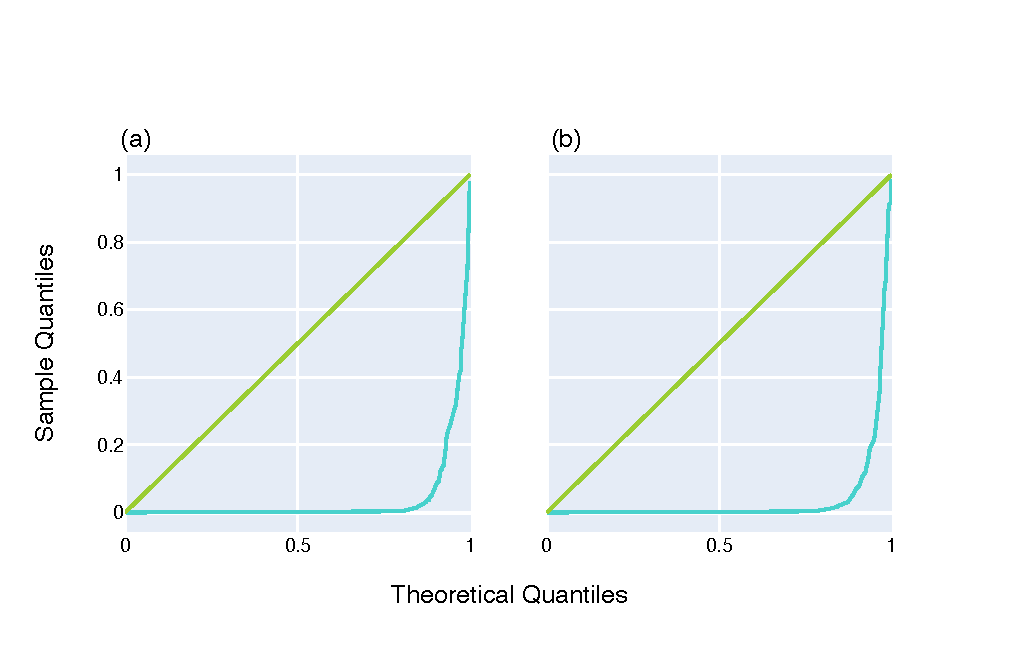
\includegraphics[width=\textwidth]{figures/plots/synthetic/chi2/197113_332182_17210.pdf}
\caption{}
\label{fig:synthetic/chi2}
\end{figure}

\bibliographystyle{apalike}
\bibliography{references}

\end{document}
